%  LaTeX 支持: latex@mdpi.com
%  如需支持,请附上所有编译所需的文件以及日志文件,并说明您的操作系统、LaTeX 版本和 LaTeX 编辑器。

%=================================================================
\documentclass[sensors,article,submit,moreauthors]{Definitions/mdpi}
\usepackage{pst-pdf}
%\documentclass[journal,article,submit,pdftex,moreauthors]{Definitions/mdpi}
%\documentclass[preprints,article,submit,pdftex,moreauthors]{Definitions/mdpi}
% 如果希望将此稿件的早期版本作为预印本发布,可以使用 "preprints" 作为期刊名称。
% 在发布前,将 "submit" 改为 "accept" 将移除行号。

%=================================================================

% MDPI 内部命令 - 请勿修改。
\firstpage{1}
\makeatletter %这段代码使用\makeatletter和\makeatother来允许使用@符号(这是使用 LaTeX 的内部命令),通过\setcounter{page}{\@firstpage}将当前页码设置为第一页面的编号。
\setcounter{page}{\@firstpage}
\makeatother

\pubvolume{1} % 期刊卷号设置为1。
\issuenum{1} %期刊期号设置为1。
\articlenumber{0} % 文章编号设置为 0,通常设置为文章唯一标识符,0 可能表示此篇文章暂未分配具体编号。
\pubyear{2025} % 出版年份和版权年份都设置为2025。
\copyrightyear{2025}
%\externaleditor{Firstname Lastname} % 外部编辑器, 可以指定外部编辑的姓名,如果有多个编辑,需要在最后一个编辑名字前后加``和''号。
\datereceived{ } % 收到稿件的日期
\daterevised{ } % 修订日期(留空,表示没有修订日期)。
\dateaccepted{ } % 接受日期
\datepublished{ } % 发布日期
%\datecorrected{} % 用于修正稿件,标明“已更正”日期。
%\dateretracted{} % 用于撤回稿件,标明“已撤回”日期。
\hreflink{https://doi.org/} % 此命令用于添加文章的 DOI(数字对象标识符)链接。
%\doinum{} % 这是用于输入具体 DOI 编号的命令,此行已被注释掉,表示暂未填写。
%\pdfoutput=1 % 这行代码指定 LaTeX 输出为 PDF 格式,适用于上传至 arXiv。如果在上传时需要,可以去掉注释。
%\CorrStatement{yes}  % 此行注明是否需要添加关于修正的信息,如果需要,可以去掉注释并填写。
%\longauthorlist{yes} % 如果文档中作者数量众多且超出默认显示范围,可以去掉注释以启用长作者列表样式。


%=================================================================
% 在这里添加宏包和命令.以下宏包已在我们的类文件中加载:
%	fontenc, inputenc, calc, indentfirst, fancyhdr, graphicx, epstopdf, lastpage, ifthen, float, amsmath, amssymb, lineno, setspace, enumitem, mathpazo, booktabs, titlesec, etoolbox, tabto, xcolor, colortbl, soul, multirow, microtype, tikz, totcount, changepage, attrib, upgreek, array, tabularx, pbox, ragged2e, tocloft, marginnote, marginfix, enotez, amsthm, natbib, hyperref, cleveref, scrextend, url, geometry, newfloat, caption, draftwatermark, seqsplit
% cleveref: load \crefname definitions after \begin{document}
% cleveref:在 \begin{document} 之后加载 \crefname 定义。 cleveref 宏包在文档的主体内容开始后加载,以确保其交叉引用功能在整体文档中正确设置。这是为了避免在没有定义引用名称的情况引用带有预定义格式的标签。
\usepackage{subcaption}

%=================================================================
% 数学环境参照: heorem, Lemma, Corollary, ...


%=================================================================
% Full title of the paper (Capitalized)
\Title{Research on Road Damage Detection in Multiple Countries Based on CAYOLO}

% MDPI internal command: Title for citation in the left column
\TitleCitation{Road Damage Detection}

% Author Orchid ID: enter ID or remove command 我没有所以不添加
% \newcommand{\orcidauthorA}{0000-0000-0000-000X} % Add \orcidA{} behind the author's name

% Authors, for the paper (add full first names)
%\Author{Firstname Lastname $^{1,\dagger,\ddagger}$\orcidA{}, Firstname Lastname $^{2,\ddagger}$ and Firstname Lastname $^{2,}$*}
\Author{Zhen Liu $^{1}$, Fei-Fan Lao $^{1}$, Sheng-Bing Che $^{1,}$*, Shuo Zhang $^{1}$,Sha Zhou $^{1}$ and Yang-Zhuo Tuo $^{1}$}

%\longauthorlist{yes}

% MDPI internal command: Authors, for metadata in PDF
\AuthorNames{Zhen Liu, Fei-Fan Lao, Sheng-Bing Che, Shuo Zhang,Sha Zhou and Yang-Zhuo Tuo}

% MDPI internal command: Authors, for citation in the left column, only choose below one of them according to the journal style
\isAPAStyle{%
    \AuthorCitation{Lastname, F., Lastname, F., \& Lastname, F.}
}{%
    \isChicagoStyle{%
        \AuthorCitation{Lastname, Firstname, Firstname Lastname, and Firstname Lastname.}
    }{
        \AuthorCitation{Lastname, F.; Lastname, F.; Lastname, F.}
    }
}

% Affiliations / Addresses (Add [1] after \address if there is only one affiliation.)
\address{%
    $^{1}$ \quad College of Computer and Information Engineering,Central South University of Forestry and Technology,ChangSha 410004,China\\
%    $^{2}$ \quad Affiliation 2; e-mail@e-mail.com
}

% Contact information of the corresponding author
\corres{Correspondence: t20050514@csuft.edu.cn}

% Current address and/or shared authorship
%\firstnote{Current address: Affiliation.}  % Current address should not be the same as any items in the Affiliation section. 上面的\dager
%\secondnote{These authors contributed equally to this work.} % 上面的\ddagger
% The commands \thirdnote{} till \eighthnote{} are available for further notes

%\simplesumm{} % Simple summary

%\conference{} % An extended version of a conference paper

% Abstract (Do not insert blank lines, i.e. \\)
\abstract{Road damage detection is an international research focus, but the accuracy of damage detection has been low due to the complexity and diversity of damage features. This paper propose a CAYOLO deep learning network model based on the CAC3 and DBC3 structures in this paper. DBC3 captures the information of slight damages, while CAC3 enables the network to focus on the features of the damage in the channel and direction. The multi-scale feature pyramid structure shortens the in-formation transmission path and makes it easier to transmit information from the bottom to the top, boosting the model's ability to extract targets at different scales. Aiming at public datasets of road damages with features of India, the Czech Republic, and Japan, the research team collected 1981 image data of Chinese road damages in diverse parts of Hunan Province, China. It detected four typical damages: D00, D10, D20, and D40. It is discovered that the CAYOLO network model suggested in this paper can enhance overall detection results in the datasets of various nations than all known network models of the same type. The average detection time for a single image is 10.2ms, the D10 AP detects Japanese images at 45.56\%, and the mAP detects Chinese images at 94.9\%.}

% Keywords
\keyword{Road damage; CAYOLO; CAC3; DBC3; deep learning}

%%%%%%%%%%%%%%%%%%%%%%%%%.


%%%%%%%%%%%%%%%%%%%%%%%%%%%%%%%%%%%%%%%%%%
% Only for the journal Data
%\dataset{DOI number or link to the deposited data set if the data set is published separately. If the data set shall be published as a supplement to this paper, this field will be filled by the journal editors. In this case, please submit the data set as a supplement.}如果论文涉及独立发布的数据集,可以提供 DOI 或者相关链接。如果数据集作为论文的补充材料一起发布,MDPI 编辑部会填写这个部分

%\datasetlicense{License under which the data set is made available (CC0, CC-BY, CC-BY-SA, CC-BY-NC, etc.)} % 数据集许可证

%%%%%%%%%%%%%%%%%%%%%%%%%%%%%%%%%%%%%%%%%%
% Only for the journal Advances in Respiratory Medicine, Smart Cities and Sensors 对于这三个期刊,我们正好是Sensors期刊
%\addhighlights{yes} % 这些期刊要求 强制填写文章亮点(highlights),用于提高搜索引擎索引和可读性:
%\renewcommand{\addhighlights}{%
%%
%\noindent This is an obligatory section in “Advances in Respiratory Medicine and Smart Cities”, whose goal is to increase the discoverability and readability of the article via search engines and other scholars. Highlights should not be a copy of the abstract, but a simple text allowing the reader to quickly and simplified find out what the article is about and what can be cited from it. Each of these parts should be devoted up to 2~bullet points.\vspace{3pt}\\
%\textbf{What are the main findings?}
% \begin{itemize}[labelsep=2.5mm,topsep=-3pt]
% \item First bullet.
% \item Second bullet.
% \end{itemize}\vspace{3pt}
%\textbf{What is the implication of the main finding?}
% \begin{itemize}[labelsep=2.5mm,topsep=-3pt]
% \item First bullet.
% \item Second bullet.
% \end{itemize}
%}

%%%%%%%%%%%%%%%%%%%%%%%%%%%%%%%%%%%%%%%%%%
\begin{document}

%%%%%%%%%%%%%%%%%%%%%%%%%%%%%%%%%%%%%%%%%%
% The order of the section titles is different for some journals. Please refer to the "Instructions for Authors” on the journal homepage.


    \section{Introduction}

    Roads play an indispensable role in every country as infrastructure that connects various parts of people's daily lives, such as schools, companies, and shopping malls. They bring great convenience to our lives and are an essential part of modern transportation systems. However, due to aging, lack of regular maintenance, and some natural causes, pavements can deteriorate and wear out to varying degrees. Road maintenance departments worldwide are faced with an increasing number of maintenance tasks. More serious, the pothole type of damage is a potential threat to the safety of people driving on the road, increasing the incidence of road accidents and may even cause severe casualties. According to the data made available by the Ministry of Transport of the People's Republic of China, although the cost of road maintenance in 2020 is 8.45 billion yuan less than in 2019, the total amount still reaches as much as 149.95 billion yuan\citep{MOT2021}. The country spends so much on road maintenance every year that it is vital to research a model that can be generalized and can accurately detect road damage.

    Many studies and investigations have been conducted into road damage in several countries\citep{miller2009crash}. Among the road damage detection methods, the most commonly used methods are manual assessment\citep{chatterjee2018fast}, semi-automatic assessment\citep{shim2022road}, and fully automatic assessment\citep{liang2022automatic}. The first approach, which primarily relies on the road assessor stepping on the road or watching the road surface from a slow-moving car, is vulnerable to traffic jams and threats to the assessor's safety. The second is a fully automatic distress assessment method with high detection accuracy. However, it needs to be equipped with expensive infrared sensor equipment, and the detection object is only cracked. The third is semi-automatic assessment, where the image collection equipment is attached to the vehi-cle and collects data while the car is in motion, while the data processing process is han-dled indoors, but it also takes much time in the data processing. Since fully automated inspection vehicles are exceedingly expensive to purchase and operate, reaching \$30--50 per kilometer\citep{radopoulou2015detection}, few national highway agencies have such fully automated inspection vehicles. However, many countries and municipalities lack the relevant technology and sufficient funds to purchase expensive devices. Roadway inspection using smartphones is becoming cheaper to execute as mobile devices like smartphones progress, many of which feature high-resolution digital cameras and processors. Puspita et al.\citep{puspita2022road} proposed to use smartphones in vehicles to obtain road images and detect road damage. In this context, developing a general road assessment model is crucial.

    In general, the following three points can be made out of this question's contributions:

    (1) The DBC3 structure was designed to extract the details of the minor cracks based on the disease's characteristics.

    (2) To maintain the feature's information in the channel and direction, two structures have been used: the feature pyramid structure and the attention CAC3 structure.

    (3) Experiments on multiple algorithms and datasets show that our proposed method can get better results.

    The structure of this paper is as follows: The second section discusses some work related to this study, the third section introduces the dataset used and the evaluation method of the experimental results, the fourth section discusses the design of the model, and the fifth section explains the experimental results and analysis, and the conclusions of the sixth section.


%%%%%%%%%%%%%%%%%%%%%%%%%%%%%%%%%%%%%%%%%%

%    \bibliography{references}


    \section{Related Work}

    \subsection{Study of Damages Based on Images Taken on the Vertical Road}

    Most of the algorithmic models were designed based on machine learning. Aravind et al.\citep{aravind2021machine} developed an advanced machine learning-based framework for concrete crack detection and failure pattern recognition, employing six classifiers to analyze experimental images of concrete beams. Their approach achieved 100\% accuracy in failure pattern identification using support vector classifiers, demonstrating superior performance in classifying flexural, shear, and compression failures. Sun et al.\citep{sun2023employing} proposed an optimized crack detection method utilizing histogram of oriented gradient (HOG) features with support vector machine classification, demonstrating superior accuracy and computational efficiency compared to conventional methods through Bayesian-optimized hyperparameter selection. De León et al.\citep{deleon2023new} developed a novel crack segmentation algorithm combining minimal path selection theory with Gabor filter-based texture analysis, achieving a competitive F1-score of 0.839 while maintaining full workflow transparency and operational flexibility across various infrastructure monitoring scenarios.


    With the proposal of deep learning neural networks, many road damages based on neural networks have emerged. Zhang et al. first used deep convolutional neural networks to bridge the gap with traffic studies, used ConvNet to compare with SVM and Boosting methods, and experimentally demonstrated that the ConvNet-based method can correctly identify the presence of cracks in pictures.
%    Xu et al.[12]\citep{xu202} proposed CrdNet, a cascaded damage detection network addressing key challenges in road damage detection through three innovative components: (1) LrNet backbone for enhanced weak semantic information representation, (2) multi-scale anchor mechanism for handling abnormal geometric properties, and (3) adaptive proposal assignment strategy for establishing range dependencies, achieving 90.92\% mAP on road damage datasets.
    Samma et al.\citep{samma2021evolving} developed an optimized VGG-19 model using a novel two-layer optimizer for drone-based road damage detection, achieving 96.4\% F1-score accuracy while reducing the number of convolutional filters by 52\% compared to the original architecture, outperforming conventional optimization methods including PSO and reinforcement learning-based approaches. Luo et al.\citep{luo2023enhanced} proposed E-EfficientDet, an enhanced lightweight network featuring a novel feature extraction enhancement module (FEEM) and semi-dense connected pyramid structures, achieving 2.41\% higher accuracy than EfficientDet-D0 while maintaining real-time performance (27.0 FPS) and compact model size (32.31 MB), suitable for deployment on mobile inspection platforms. He and Chen\citep{chen2022novel} introduced a new neural network for road crack detection, AttentionCrackNet, which uses an encoder-decoder structure and inserts an attention mechanism named the attention gate, which enables the network to focus more on crack features.


    However, the two critical features of weak semantic information and geometric feature anomalies are not considered in most CNN-based road crack detection studies. Xu, Chen, and Qin\citep{xu2021cnn} accordingly proposed CrdNet, a backbone consisting of LrNet\citep{sun2021improving} with the addition of a multiscale aspect ratio mechanism, length awareness, and a cascade detection head, and demonstrated that using the CrdNet network to detect pavements can achieve better results than the Faster R-CNN algorithm\citep{ren2015faster}, and mAP can reach 90.92\%. Dorafshan et al.\citep{dorafshan2018comparison}, who compared several common edge detectors and neural network models AlexNet DCNN\citep{lecun1998gradient}, discovered that the deep learning-based approach outperformed various edge detection methods to detect cracks smaller than 0.04 mm. However, DCNN takes more time to acquire pre-trained models. Kulambayev et al.\citep{kulambayev2023real} introduced an optimized Mask R-CNN framework for real-time road surface damage detection, demonstrating superior accuracy and computational efficiency in detecting various road aberrations including cracks, potholes, and rutting across diverse environmental conditions. Hacıefendioğlu and Başağa\citep{haciefendiouglu2022concrete} developed a comprehensive crack detection system using Faster R-CNN, achieving robust performance across varying weather conditions and illumination levels, with detailed analysis of detection rates under different environmental scenarios including sunny, cloudy, and foggy conditions, as well as sunset and moonlight periods.


    Although studies using images taken vertically to the road surface can produce good detection results, studies using such images have several limitations: the expense of regularly collecting new images using specialized vehicles is too high; the collected images do not cover the entire road surface, and the constructed models of this type are better suited for dealing with classification problems. Due to these problems, disease studies based on images taken from dashboards have emerged.

    \subsection{Study of Damages Based on Images Taken on the Dashboard}


    The second kind of detection study is the semi-automatic assessment approach discussed in the first section, which uses a smartphone fixed to the dashboard or windshield to take pictures and then performs image processing and detection model building in the room. In addition to the road, the photos obtained using this method also include distracting things like trees, buildings, and automobiles, which makes it challenging to detect pavement illness. Despite these limitations, this study is made possible because it only needs a smartphone to gather the photographs, and the research data may be easily updated.

    In 2018, public datasets of these photographs were made available, and most of them were analyzed using deep learning techniques. Road damage types were divided into eight categories by Maeda et al.\citep{maeda2018road} in 2018, trained on the eight categories using SSD Inception V2[23, 24]\citep{szegedy2016rethinking,liu2016ssd} and SSD MobileNet\citep{howard2017mobilenet}, resulting in recall and precision rates of 71\% and 77\%. The dataset, RDD-2018, was collected using cell phones placed on windshields. Wang et al.\citep{wang2018road} conducted experiments using SSD and Faster R-CNN based on the dataset RDD-2018 and performed data augmentation operations with brightness adjustment and Gaussian blurring, and the F1-score reached 0.6255. Wang et al.\citep{wang2018deep} fused 14 base models using pre-trained ResNet\citep{He_2016_CVPR} and VGG\citep{vgg} as the backbone to handle damage detection and classification tasks to enhance the performance of the models. Chen et al.\citep{chen2020road} trained Mask R-CNN\citep{He_2017_ICCV} with DenseNet\citep{Huang_2017_CVPR} as the backbone, used a feature pyramid network combined with multi-scale features for detection, and used Labelme to polygon label the identified diseases again based on RDD-2018.
%    In the 2018 IEEE road damage detection and classification challenge, Alffrrarjeh et al.[33] improved and cropped eight different types of photos with an F1-score of 0.62 using the YOLOv3[34].
    To improve the F1 score, Maeda et al.\citep{maeda2021generative} first cropped the damaged part of the D40 category into pixel blocks, then generated more pothole-type diseases using PG-GAN\citep{karras2018progressive}, and finally combined the generated images with non-damage images using Poisson fusion. When there were fewer original images, the F1 score increased by 5\%, and the F1 score increased by 2\% when the number of training images was increased. Additionally, the authors proposed RDD-2019 based on RDD-2018, which meant that the annotations of the RDD-2018 dataset were updated and expanded in number. To increase the precision of local bounding boxes in the dataset, Yin et al.\citep{yin2021road} suggested a multilayer feature pyramid method based on M2det\citep{zhao2019m2det} with an attention mechanism.


    Arya et al.\citep{arya2021rdd2020} created RDD-2020 by combining road pictures from the Czech Republic and India with the Japanese dataset to identify cracks and potholes. This dataset was based on RDD-2019. Additionally, they examined how changing the number of training photographs affected the model's performance. The trials revealed that using more training images improved the model's performance.
%    Mandal et al.[40] use the transfer learning method to compare the one-stage and two-stage algorithm models. YOLO can achieve better results than CenterNet[41] and EfficientDet[42], achieving an F1-score of 0.5814 and 0.5751 on test1 and test2, respectively, and fourth place in the IEEE Global Road Damage Detection Challenge 2020. Nsddaf-Sh et al.[43] used EfficientDet to detect damages and found a contradiction between better real-time performance and accuracy in the detection process. Pham et al.[44] used Detectron2 to improve the training speed of Faster R-CNN, cropped down the labeled diseases to improve the detection performance of the model, flipped, rotated, and scaled the cropped images horizontally, and finally manually placed the processed images into the images using color conversion technique. The final F1-score reached 0.51 and 0.514, but the training speed is slow, and the prediction time is also longer.
    Chen et al.\citep{chen2023research} developed an optimized YOLOv5-based road damage detection system using the RDD-2020 dataset, implementing a comprehensive data preprocessing pipeline to address labeling inconsistencies and achieving efficient real-time detection capabilities for both damage localization and classification. Hasan et al.\citep{hasan2022road} conducted extensive experiments with five pre-trained models on the RDD-2020 dataset, proposing a fine-tuned Faster RCNN with ResNet-101 architecture that achieved improved F1-scores of 0.47, 0.41, 0.41, and 0.35 for longitudinal cracks, transverse cracks, alligator cracks, and potholes respectively, outperforming previous approaches in detecting overlapping damage regions. Wu et al.\citep{wu2024utilize} proposed Flexi-Weather Hard Detection, an innovative algorithm integrating AIGC-based data augmentation and corner point feature aggregation, achieving 64.9\% in Test1 metric and 40.6\% F1-Score on RDD-2020 and CNRDD datasets, with enhanced robustness in adverse weather conditions through Weather Trim Augment module and improved local feature learning via Flexi Corner Block.
    % 注意,CNRDD没有引用.[44]是preprint,可以改成:https://link.springer.com/chapter/10.1007/978-981-99-8549-4_13



    Shim et al.\citep{shim2021road} designed a disease segmentation block with four dense blocks containing encoders and decoders based on DenseNet-121 to achieve an F1-score of 79.33 with only 3.56M parameters. However, the algorithm only detects the presence of damage in the images. Lin et al.\citep{lin2021implementation} performed road picture capturing from two angles, 70° and 30°. They collected 620,000 damages in Taiwan, China, and classified the damages into six categories, taking utility hole covers and repairs into consideration. They conducted experiments using YOLOv3 and achieved 71\% accuracy in detecting pothole-type damages. Rehana et al.\citep{rehanak2022road} applied only 2607 photos to train the network to detect seven damage categories, with a 92\% overall accuracy rate. Su et al.\citep{su2022fsrdd} introduced the FSRDD model to remove redundant information and extract features by ghost attention and proposal feature metric, show the method’s applicability through ablation experiments, and reach an mAP of 51.7\% on public datasets. Chen et al.\citep{chen2024lag} proposed LAG-YOLO, a lightweight attention-based YOLO variant for road damage detection, achieving 52.35\% mAP on RDD-2020 dataset with only 4.19 million parameters through the integration of an attention ghost module and SimAM mechanism, demonstrating superior efficiency and accuracy for real-time processing and lightweight deployment. Deepa and Sivasangari\citep{deepa2023effective} developed a hybrid deep learning framework combining adaptive density-based fuzzy c-means clustering with a novel Hybrid Deep Capsule Autoencoder-based Convolutional Neural Network (Hybrid DCACN), achieving 98.815\% accuracy on the RDD-2020 dataset through an optimized feature extraction pipeline incorporating Laplacian edge detection and hybrid wavelet-Walsh transform. Rakshitha et al.\citep{rakshitha2024deep} conducted comprehensive experiments with deep CNN and ResNet architectures on the RDD2022\citep{arya2022rdd2022} dataset, demonstrating that ResNet152 achieved superior performance with an F1-score of 0.6954 through advanced data augmentation techniques including contrast transformation and Gaussian blur, outperforming ResNet50 and ResNet101 models in pavement damage classification.

    % RDD2022还没有引用

    Road damages are today the focus of numerous studies, and many solutions have been proposed. Nonetheless, few studies report the disease as a binary classification problem by masking and labeling it, which can only establish whether a disease exists. The different damage kinds, however, cannot be classified. Although the properties of the cracks have always been unclear, several studies are suggested for their extraction. Other network models have been explored by researchers to extract disease features. Two-stage networks have a long training period yet have good detection accuracy. Single-stage models take less time to train but are less accurate. In this study, several typically used object detection methods are compared. The network model CAYOLO put forward in this research stands out from the mass and achieves the best detection speed and accuracy. CAYOLO outperforms other evaluation parameters. Although CAYOLO can produce excellent results, it still misses detections during testing, leaving much space for performance enhancement.


    %%%%%%%%%%%%%%%%%%%%%%%%%%%%%%%%%%%%%%%%%%


    \section{Datasets and Methods}

    \subsection{Datasets}

    The dataset used in this paper was provided by the 2020 IEEE Big Data Road Damage Detection Challenge[35, 53-55]\citep{maeda2021generative,arya2021deep,arya2021rdd2020,arya2020global}. The images in this dataset were captured with a smartphone fitted to the dashboard or windshield of a car. The dataset mainly includes images from Japan, the Czech Republic and India, and the official dataset was divided into one training set and two test sets. The labeling file of the training set was PASCAL VOC format and included unified names for various types of damage. Due to privacy reasons, only the annotation files of the training set are officially disclosed, so this paper only uses the data provided in the training set for experimental research.

    \begin{figure}[H]
        \centering
        \subfloat[\centering Japan road]{
            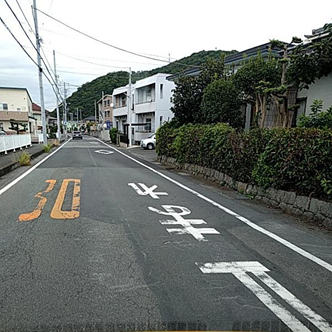
\includegraphics[width=0.45\textwidth]{images/figure1-a}
        }
        \hfill
        \subfloat[\centering Indian road]{
            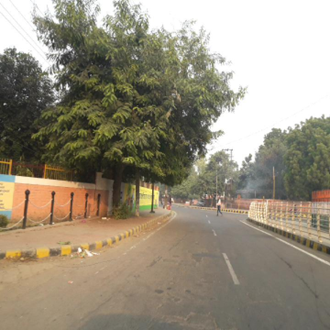
\includegraphics[width=0.45\textwidth]{images/figure1-b}
        }\\
        \subfloat[\centering Czech road]{
            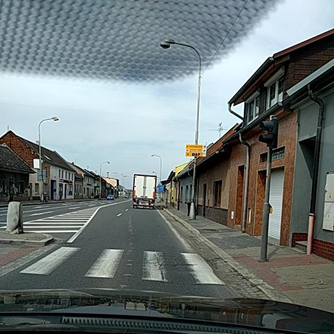
\includegraphics[width=0.45\textwidth]{images/figure1-c}
        }
        \hfill
        \subfloat[\centering China road]{
            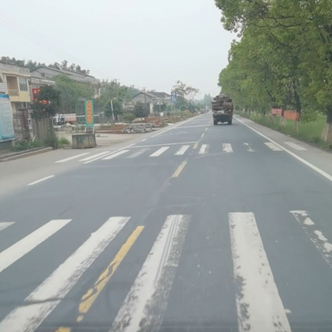
\includegraphics[width=0.45\textwidth]{images/figure1-d}
        }
        \caption{Examples of road pictures from several countries.\label{fig:1}}
    \end{figure}

    Since the data provided in the 2020 challenge mainly identifies and detects four categories of road damages: longitudinal cracks(D00), transverse cracks(D10), alligator cracks(D20), and potholes(D40), as shown in~\autoref{tab:1}, this paper also addresses these four categories of damage that were tested. In addition, since the surface conditions of roads vary significantly from country to country, as shown in~\autoref{fig:1}, there are considerable differences between Indian roads and the rest of the nations. The number of Japanese datasets is the largest, with only the training set images provided by the public dataset being used for experiments in this thesis. The five categories that are not considered are dropped. There are a total of 7900 images containing damage in the end, and the training set, validation set, and test set are divided according to the ratio of 8:1:1. The number of training sets, verification sets and test sets were 6320, 790 and 790 images respectively.

    \begin{table}[H]
        \caption{Damage types and illustrations.\label{tab:1}}
        \begin{tabularx}{\textwidth}{>{\centering\arraybackslash}m{4cm}>{\centering\arraybackslash}m{4cm}>{\centering\arraybackslash}m{5cm}}
            \toprule
            \textbf{Damage Name} & \textbf{Damage Type}                 & \textbf{Damage Detail Illustration}          \\
            \midrule
            D00                  & Longitudinal cracks                  & 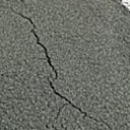
\includegraphics[width=2cm]{images/table1-1} \\
            D10                  & Transverse cracks                    & 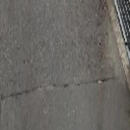
\includegraphics[width=2cm]{images/table1-2} \\
            D20                  & Alligator cracks                     & 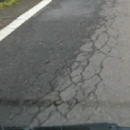
\includegraphics[width=2cm]{images/table1-3} \\
            D40                  & Potholes, bumps, rutting, separation & 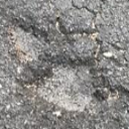
\includegraphics[width=2cm]{images/table1-4} \\
            \bottomrule
        \end{tabularx}
    \end{table}


    Meanwhile, this study collected data on partial highways and urban roads throughout Hunan Province, China, using smartphones placed on the dashboard, and the collected data size was $1920\times1080$. The image size was adjusted to a uniform $600\times600$ after processing, consistent with the publicly available RDD-2020 dataset. When labeling the data, nine damage types were labeled according to the criteria given in the public dataset, but only four damage types were used for the experiment, and the data is presented in \autoref{tab:3}, with a total of 1981 images and 2551 damages. The number of various damage types in each country is listed in detail in \autoref{tab:2}, and it can be noted that Japan has the most significant total number of D20 categories and relatively few D40 types; India has a severe imbalance in the data of various kinds of damage, with only 60 D10 categories; and there is also an inbalance in the Czech Republic and China. From the given data, it is apparent that there are significant variations in each country’s scenario, making it imperative to research a detection model that is widespread worldwide.

    \begin{table}[H]
        \caption{A number of road damage data by category in a different countryt.\label{tab:2}}
        \begin{tabularx}{\textwidth}{LCCCC}
            \toprule
            & \textbf{D00} & \textbf{D10} & \textbf{D20} & \textbf{D40} \\
            \midrule
            Japan & 3644         & 3577         & 5590         & 2061         \\
            India & 1388         & 60           & 1827         & 2852         \\
            Czech & 892          & 352          & 136          & 175          \\
            China & 749          & 926          & 193          & 683          \\
            \bottomrule
        \end{tabularx}
    \end{table}

    Even though this study only collected a limited number of photographs compared to that public dataset, the D10 category with less obvious damage characteristics received relatively more data. We carefully comply with the criteria during the labeling process and repeatedly examine the labeled dataset to avoid false detection and missed detection. As shown in \autoref{fig:2}, while even human eyes can recognize erroneous labeling immediately, learning models find it challenging to do so. Additionally, we strive to alter the damage's features while labeling it so that as little noise as possible enters the groundtruth bounding box.

    \begin{figure}[H]
        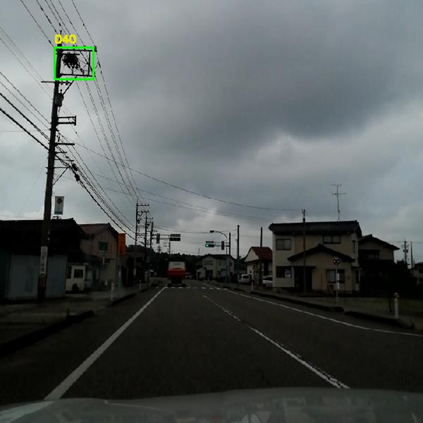
\includegraphics[width=7cm]{images/figure2}
        \caption{Error-tagging.\label{fig:2}}
    \end{figure}

    \subsection{Methods}

    Four traditional road damage types are chosen as detection targets in this work. The YOLOv5 network meets the detection requirements well and is vulnerable to problems like the overfitting phenomena and poor detection performance because pavement cracks are thin and challenging to differentiate compared to many other objects, and the amount of available datasets is constrained. On this basis, this study proposed the CAYOLO model, which can effectively address these problems.

    \subsubsection{Design of CAC3 Module}

    The Coordinate Attention Concentrated-Comprehensive Convolution(CAC3) module, a lightweight attention module with Coordinate Attention(CA)\citep{Hou_2021_CVPR}, is embedded into the C3 structure, which divides the channel attention into two one-dimensional feature coding processes for feature aggregation in different spatial directions, allowing the network to acquire long-term information in one direction and retain location information in the other direction, followed by encoding the generated feature maps separately to generate a pair of feature maps interesting in direction and location.

    \begin{figure}[H]
        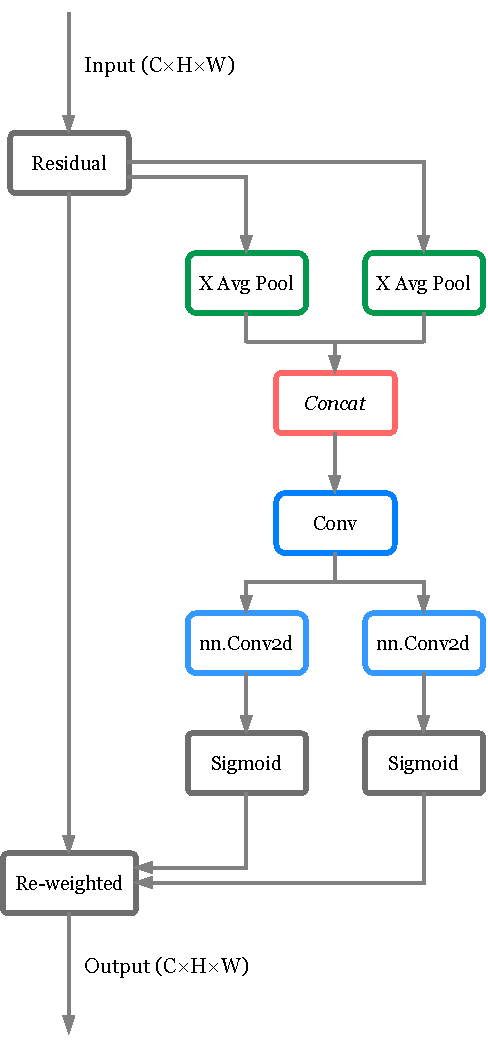
\includegraphics[width=7cm]{images/figure3}
        \caption{Error-tagging.\label{fig:3}}
    \end{figure}

    The CA attention mechanism is shown in \autoref{fig:3}. The attention module can capture the feature information in spatial order thanks to the adaptive averaging pooling operation in the horizontal and vertical dimensions. Subsequently, the two feature maps are concatenated in the channel orientation operation, followed by encoding the spatial information of the just generated feature maps with 1$\times$1 convolution and then tensor transforming the feature information in the horizontal and vertical directions using 1$\times$1 convolution, respectively, to obtain feature maps that are sensitive to the location information. The computational cost and model complexity can be efficiently reduced by CA attention since it mainly utilizes 1×1 sized convolution kernels and divides the number of channels by the scale factor (the default is 32) before implementing the first convolution.
    SENet attention\citep{Hu_2018_CVPR} operates on channels, so it focuses more on inter-channel correlation; CBAM attention\citep{Woo_2018_ECCV} uses large-size convolution to obtain location information, but it focuses less attention on channel information; while CA attention is used in this experiment, it can extract not only inter-channel information but also direction and location information, effectively improving the model's ability to locate and identify damages.
    This paper proposes a CAC3 structure, which embeds CA attention into the Bottleneck structure of the C3 architecture, as shown in the figure. During the computation of the Bottleneck, the input information is divided into g groups for processing, and residual structures with convolution kernels of size 1×1 and 3×3 are used for feature extraction. The residual structures are repeated n times, and the CA attention mechanism is added without changing the size and number of channels of the feature map. When the residual structure in the Bottleneck structure extracts deep-level information, the attention mechanism transmits the extracted spatial and positional information to the Bottleneck, which can effectively alleviate the problem of gradient vanishing. Additionally, the CAC3 structure pays more attention to the texture direction and position information of road damage during the backbone phase of the network, which can effectively extract the feature information of road damage. Experimental results show that this method can significantly improve the performance of the network and achieve good detection results.

    \subsubsection{Design of DBC3 Module}


    According to the slender traits of pavement cracks, this study designs the Double Bottleneck Concentrated-Comprehensive Convolution module(DBC3) in the neck region of the CAYOLO backbone network to extract the details of the damage and designs the Double Bottleneck inserted into the C3 structure with the convolution kernel size set to 1×1, 3×3, and 5×5, respectively. The small convolution kernel is more sensitive to slight cracks and potholes features during the training process. After Conv1, the feature vector obtained is inputted into the Double Convolution structure. Before that, the channel number is divided into two and inputted into two residual structures. The 1×1 and 3×3 small convolutions extract texture features of cracks and pits, while the 5×5 convolution focuses on the larger mesh crack features. The feature mapping network deepens the network's ability to extract deep features, and the Double Convolution structure does not cause network degradation due to the deep layers. The double convolution Double Bottleneck structure is shown in \autoref{fig:4}.

    \begin{figure}[H]
        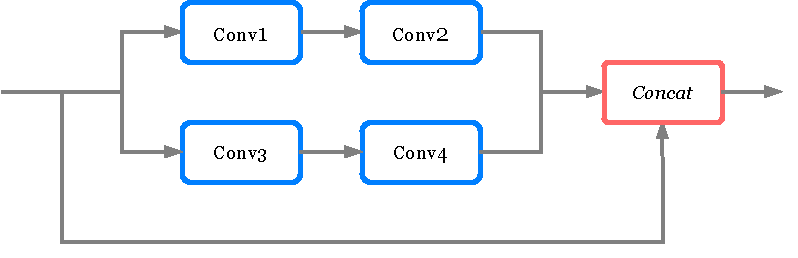
\includegraphics[width=0.8\textwidth]{images/figure4}
        \caption{The Double Bottleneck module.\label{fig:4}}
    \end{figure}


    After embedding the Double Convolution structure into the C3 structure, in order to prevent the image size from decreasing during the convolution operation and to avoid losing pixel information at the edge of the image, automatic padding is performed during the convolution operation.

    Afterward, the feature maps obtained are stacked on the channel axis. After the Double Convolution operation, some feature information may be lost and the network may suffer from model degradation due to its depth. Therefore, a shortcut operation is performed after the stacking operation to preserve the feature information of the disease. Although the addition of the Double Convolution operation may increase some computational complexity, it can improve the network's attention to small targets, so the computational complexity it brings is acceptable.

    \begin{figure}[H]
        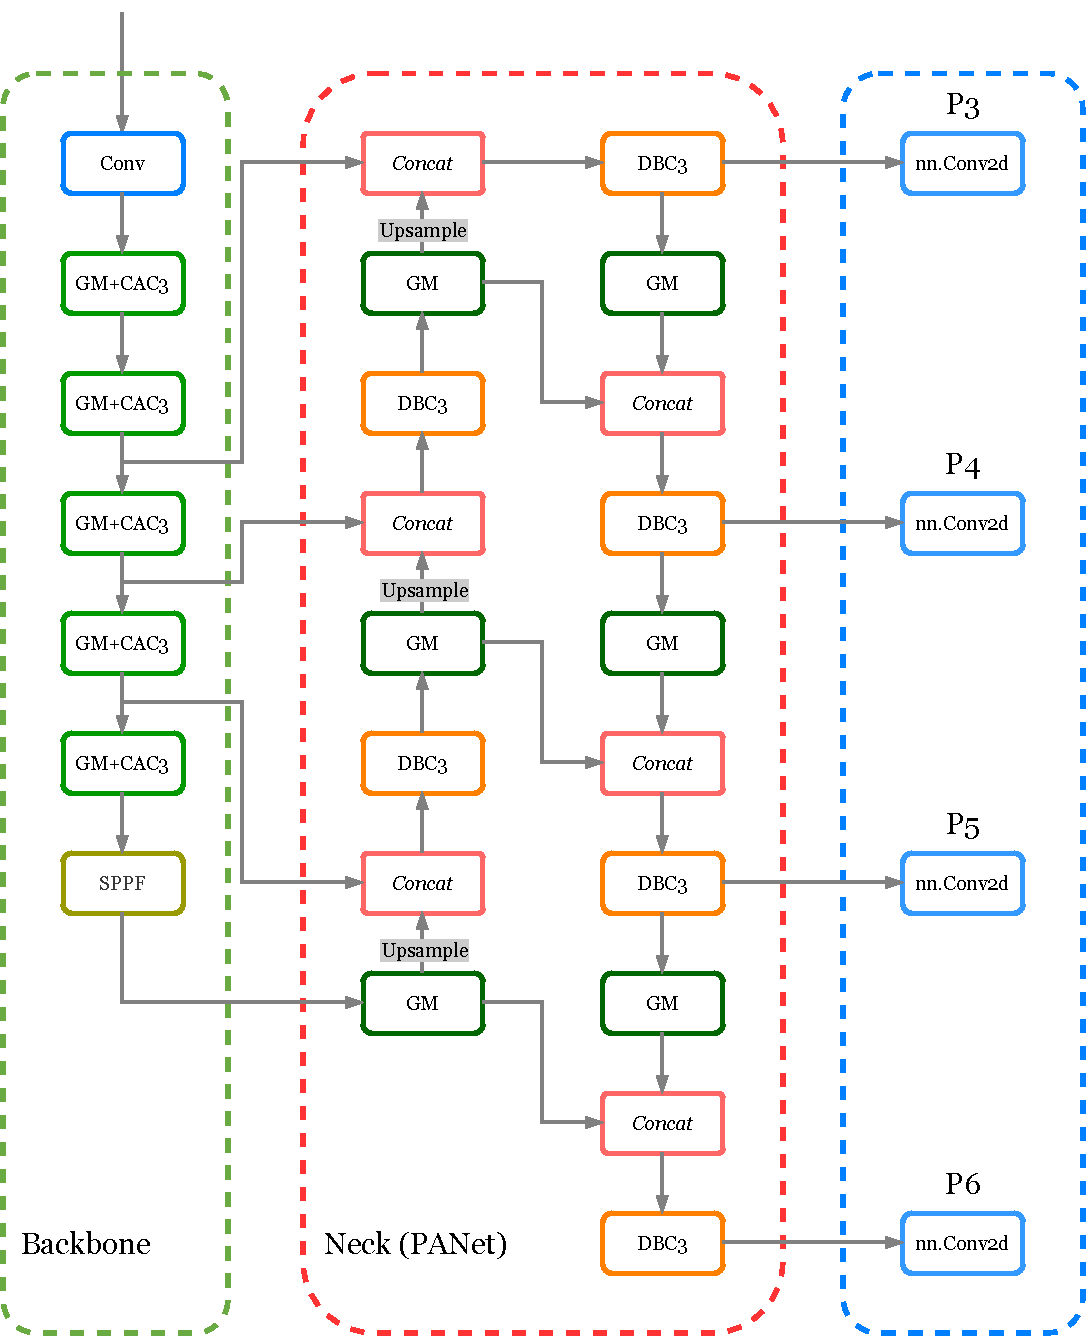
\includegraphics[width=\textwidth]{images/figure5}
        \caption{CAYOLO network structure.\label{fig:5}}
    \end{figure}


    CAYOLO's backbone structure is shown in \autoref{fig:5}. The PANet\citep{liu_2018_CVPR} structure enhances the whole feature hierarchy with accurate localization signals in the lower layers through top-down path augmentation, which shortens the information path between the lower and top layer features. Shallow feature maps have small receptive fields, contain more location information, have a strong ability to capture geometric capability, and are more suitable for detecting small targets. Deep feature maps have more robust semantic information but are more suitable for detecting large targets due to their poor detail perception ability for low-resolution images.

    The GM in \autoref{fig:5} stands for Ghost Module\citep{Han_2020_CVPR}. The bottom-up structure of PANet is the bottom-up structure of PANet is primarily introduced to preserve the vital shallow feature information of the network. After all, the shallow features contain much information, such as edge geometry, since instance segmentation is based on pixel-level classification, preserving more shallow features through this bottom-up process is beneficial, and more shallow features can be conserved after this bottom-up process. Considering the comprehensive damage characteristics, the damage targets of potholes and crack classes are small. At the same time, some of the D20 types damages have a more comprehensive range of damage, so the feature layers [P3, P4, P5, P6] are used in this experiment to detect damage targets of potholes and crack classes, which are small in size, as well as some of the D20 types that have a more comprehensive range of damage.

    %%%%%%%%%%%%%%%%%%%%%%%%%%%%%%%%%%%%%%%%%%


    \section{Evaluation}


    Model performance is estimated by two metrics, average precision(AP) and mean average precision(mAP), F1-Score. Since the classification is imbalanced in the dataset and accuracy-based metrics alone may be biased, mAP is used as the primary criterion for comparing the performance of different models in this paper, and it can be used to assess the risk of incorrect classification by using a confidence score assigned to each detected bounding box.

    The precision rate P represents the percentage of correctly predicted instances to the total number of predicted features, and the recall rate R represents the percent of correctly predicted features to the total number of features present in the actual class. Both precision rate and recall rate are based on IoU, which is the ratio of the area of overlap of the region between the predicted border and the actual edge to the area of its conjunctive region, and the IoU threshold is set to 0.5 in this paper. Where the precision and recall rates are computed as follows:

    \begin{align}
        P &= \frac{TP}{TP+FP} \\
        R &= \frac{TP}{TP+FN}
    \end{align}
%    where TP is the number of true positive samples, FP is the number of false positive samples, and FN is the number of false negative samples. The F1-Score is the harmonic mean of the precision and recall rates, and the formula is as follows:
    Among these, $TP$ means the number of damages that were accurately identified (true positives), and FP denotes the number of damages that were mistakenly identified as damages (false positives). $FN$ is the count of damages identified as non-damages (false negatives).
    The formulas for AP, mAP and F1-Score are as follows:

    \begin{align}
        AP &= \frac{1}{m} \sum_{r \in \{0.0, 0.1, \ldots, 1.0\}} P_{\mathnormal{interp}}(r) \\
        mAP &= \frac{1}{N} \sum_{i=1:n}^{N} {AP}^i \\
        F1 &= 2 \times \frac{P \times R}{P+R}
    \end{align}
    Among them, $P_{\mathnormal{interp}}(r)$ is the maximum accuracy rate by a certain condition. ${AP^i}$ is the average precision value of the i-th. The higher the $AP$ value, the better the model performance. $m$ is made up of 11 equally spaced numbers in the range $[0.0,0.1, \ldots, 1.0]$, where $n$ is the total number of categories.


    %%%%%%%%%%%%%%%%%%%%%%%%%%%%%%%%%%%%%%%%%%


    \section{Experimental Results}

    \subsection{Performance Comparison of Different Optimizer}

    This experiment was trained for 500 epochs, and \autoref{fig:6} depicts the curve of the change of the mAP value of the model during the training process. From the figure, we can see that about the 200th epoch, the network has stabilized, and the value of CAYOLO proposed in this paper is marginally higher than that of the original YOLOv5. In about 400 epochs, YOLOv5 begins to exhibit the overfitting phenomenon, and the value of mAP has a significant downward trend.

    Additionally, the network's effects of the SGD and Adam optimizers were investigated. As seen in \autoref{fig:7}, although using the SGD optimizer can bring the network to equilibrium faster, the network achieves more stable performance with less fluctuation in detection values when using the Adam optimizer, and the network is more prone to overfitting when using the SGD optimizer. This situation is likely caused by the network training for too long, the parameters updating too frequently, and the existence of noise or outliers in the training data, which leads to the occurrence of overfitting. As a result, this study uses the Adam optimizer based CAYOLO to conduct experimental work.

    \begin{figure}[H]
        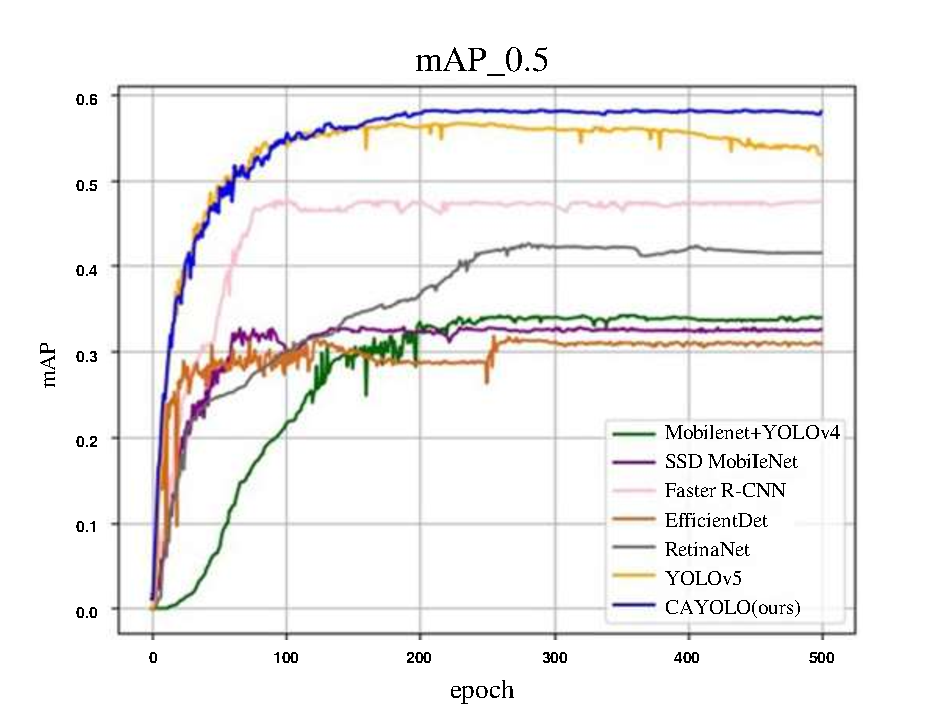
\includegraphics[width=0.8\textwidth]{./images/figure6}
        \caption{Comparison of the mAP training process of the different algorithms.\label{fig:6}}
    \end{figure}
    \unskip
    \begin{figure}[H]
        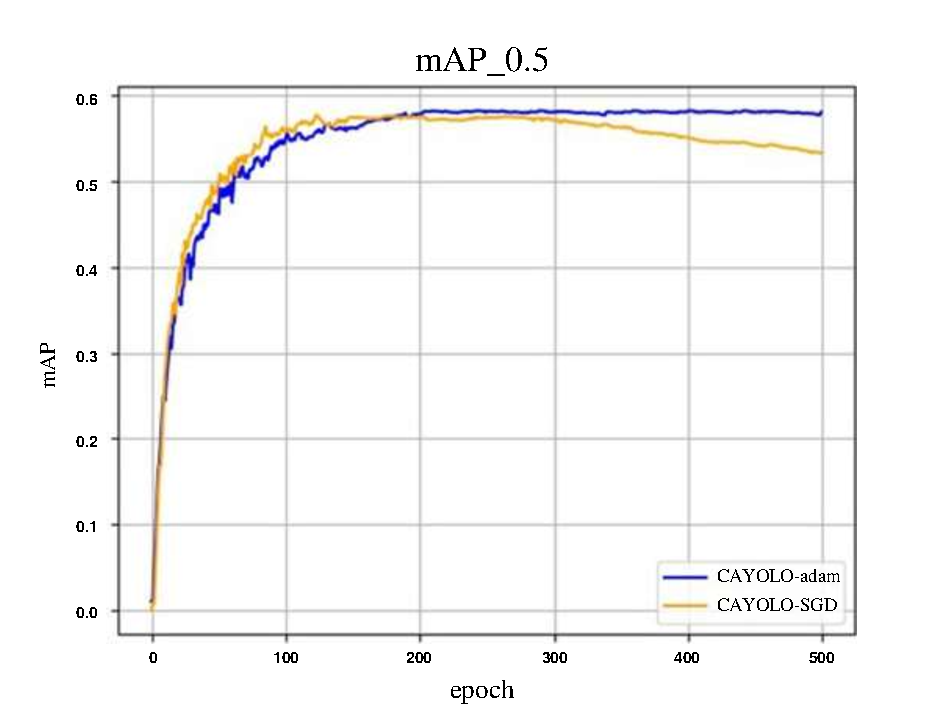
\includegraphics[width=0.8\textwidth]{./images/figure7}
        \caption{mAP changes during training with different optimizers.\label{fig:7}}
    \end{figure}

    \subsection{Comparison of Results of Different Detection Algorithms}

    To demonstrate the advantages of the model proposed in this paper, the model CAYOLO in this paper is experimentally compared with Faster R-CNN, RetinaNet, EfficientDet, MobileNet+YOLOv4, SSD MobileNet, and YOLOv5. \autoref{fig:8} shows the test set's average precision results for detection using various algorithms.

    Analyzing the information in \autoref{fig:8} demonstrates how the suggested methodology in this research can produce better outcomes for the detection of each category. The two-stage networks, Faster R-CNN and MobileNet+YOLOv4, showed comparable performance to the YOLOv5 network for detecting the D20 category. Neither EfficientDet nor SSD MobileNet showed good performance in detecting each category, the mAP of EfficientDet for the D10 was only 8.5\%. RetinaNet shows that D40 performs dramatically better than SSD MobileNet, while other categories also perform as well as SSD MobileNet. CAYOLO improved the outcomes of YOLOv5 for detecting the D20 and D40 classes. The graphs show that each network's detection performance for the D10 category is less than ideal. This phenomenon is likely due to several factors, including the D10 category's limited data supply, the lack of evident fracture features in the images, and the network's difficulty in learning the characteristics of lateral cracks.

    \begin{figure}[H]
        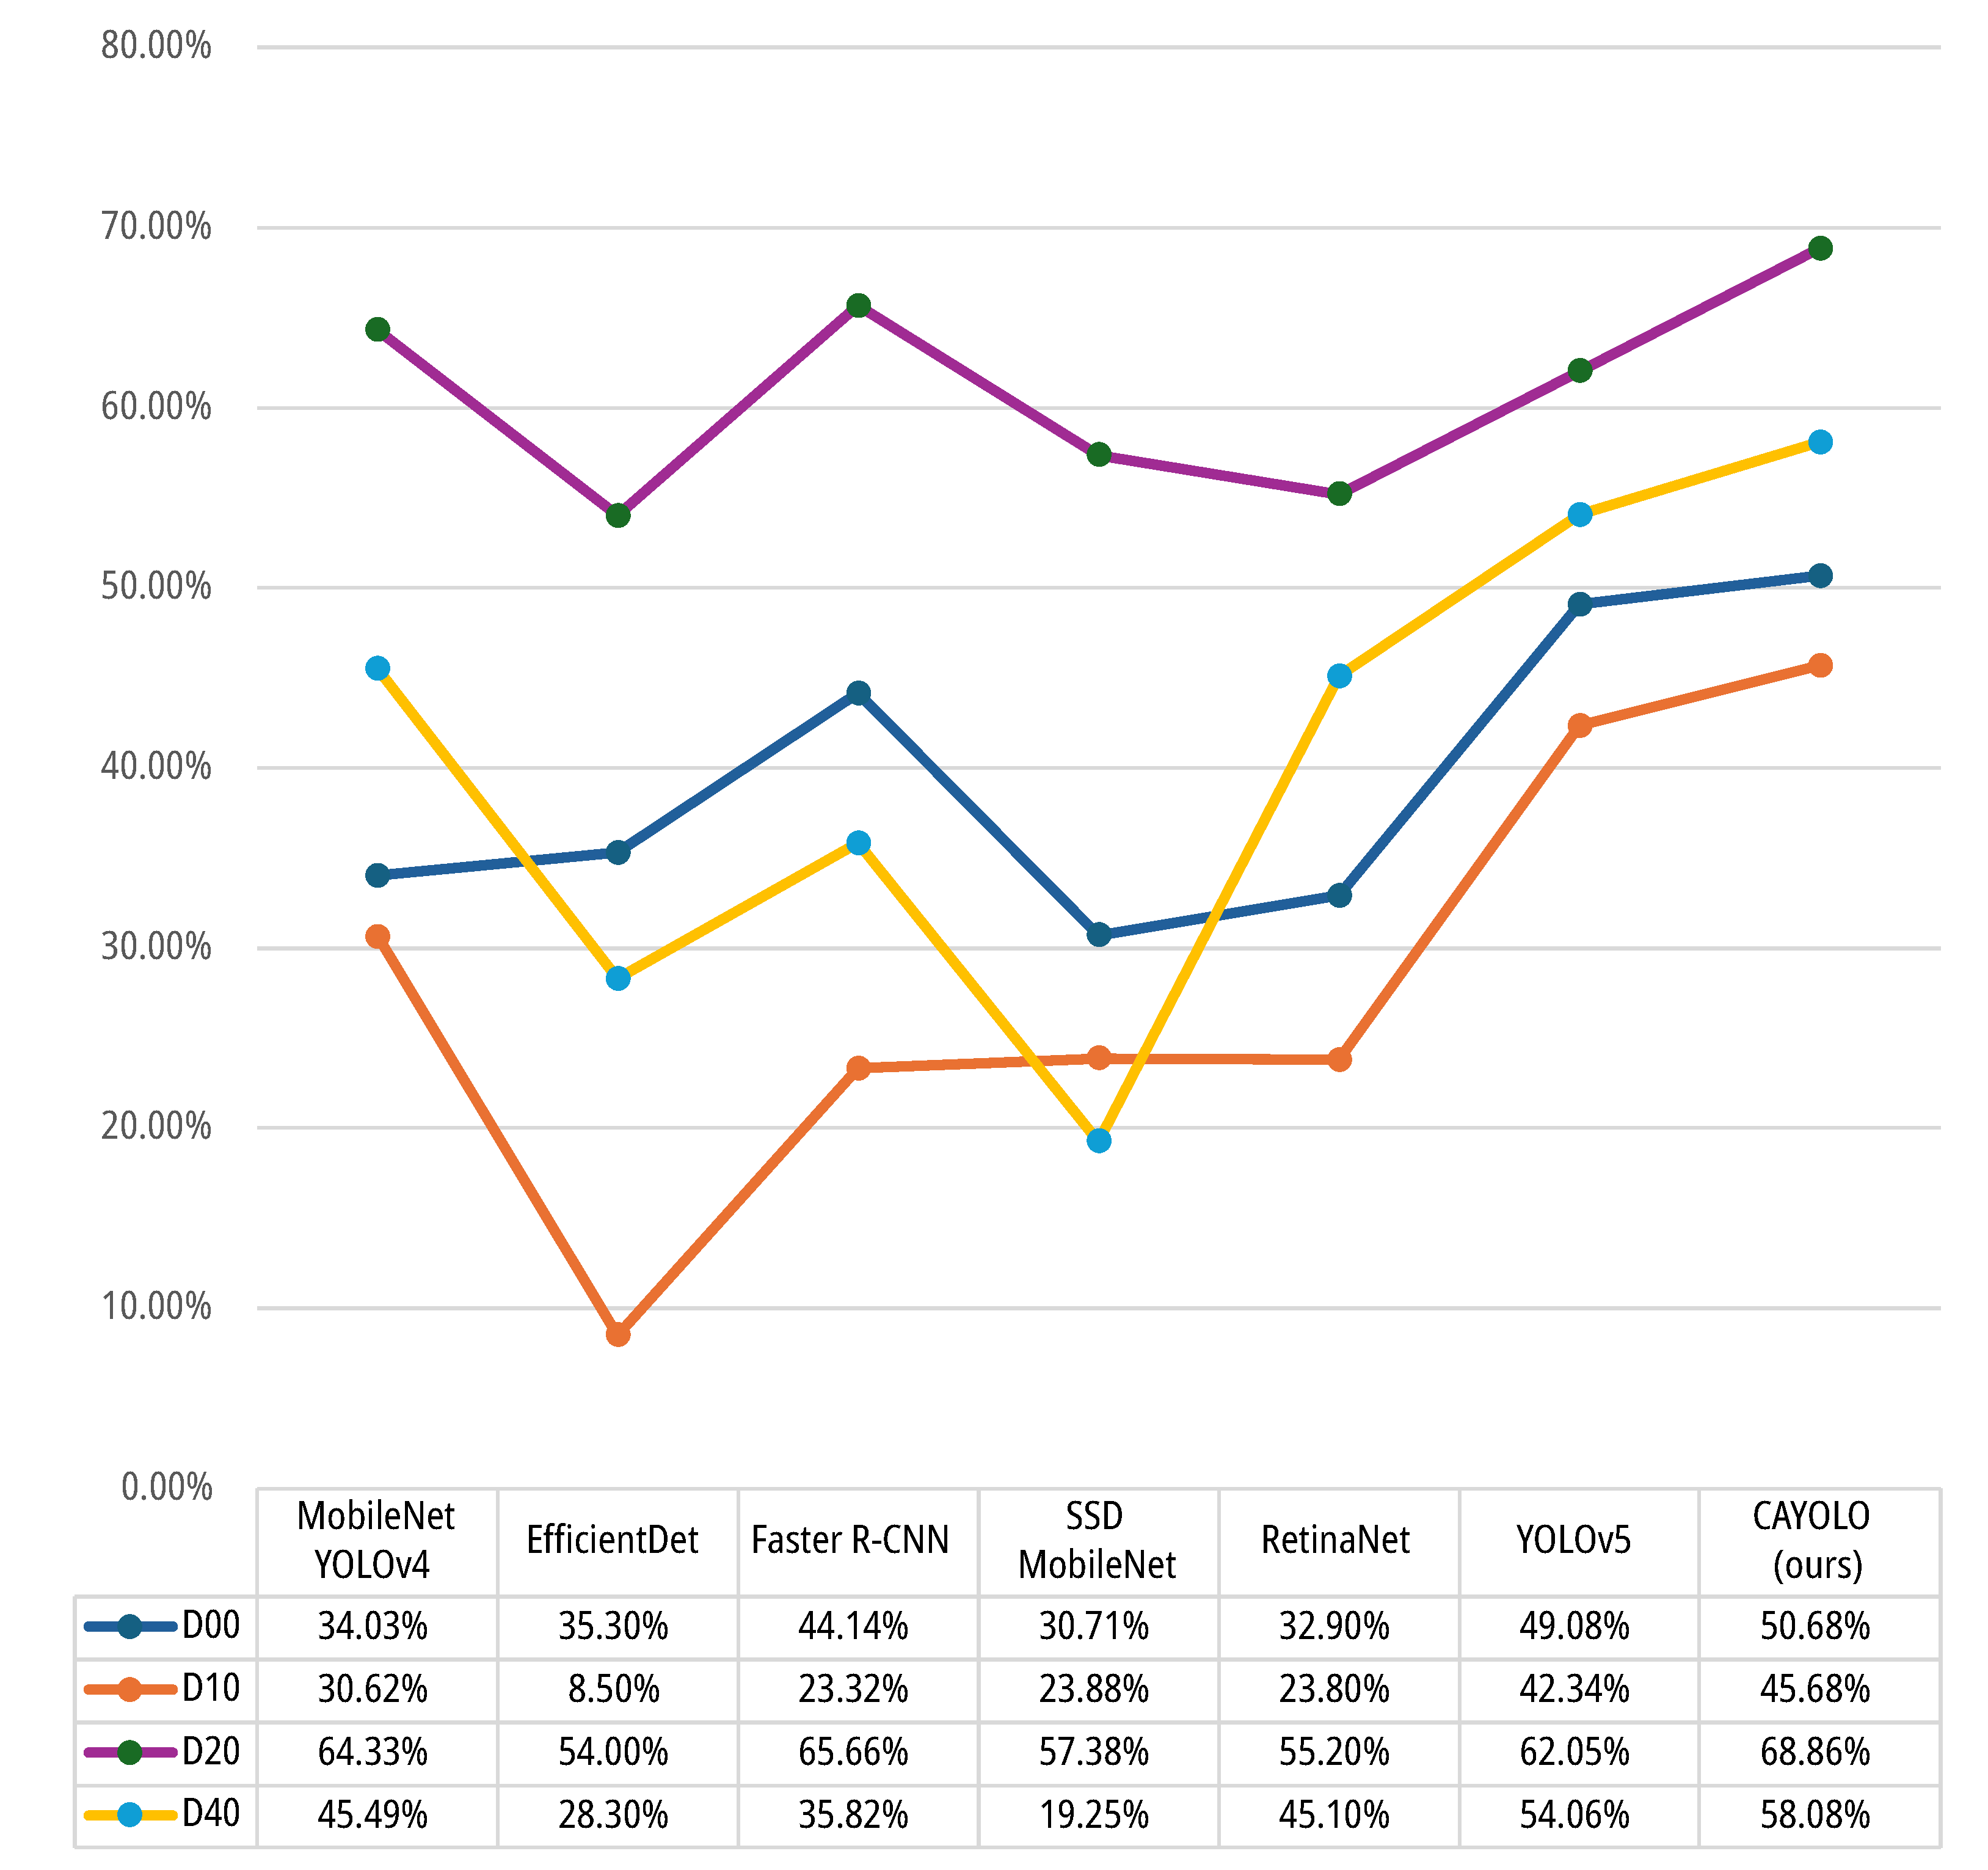
\includegraphics[width=\textwidth]{./images/figure8}
        \caption{AP values for different networks per category.\label{fig:8}}
    \end{figure}

    \autoref{fig:9} shows the evaluation of the test set using several algorithms to examine the performance of the training model. The major problem with MobileNet+YOLOv4 is that it missed all D40 and D10 class damages, as demonstrated in Figure~\autoref{fig:9-a} and Figure~\hyperref[fig:9-c]{9(c)}. In Figure~\hyperref[fig:9-a]{9(a)}, it shows that EfficientDet incorrectly classifies the object on the side wall as class D00, and Figure~\hyperref[fig:9-b]{9(b)} misidentifies D01 as class D00 damage, which is the part of the longitudinal joint between the concrete during the construction of the road. This misidentification phenomenon also exists in Faster R-CNN and YOLOv5, and in Figure~\hyperref[fig:9-c]{9(c)} also misses multiple instance of class D10 damages and misidentifies the gutter cover as D20 damage. Faster R-CNN has the highest detection accuracy; D40 is missed in Figure~\autoref{fig:9-a}, while D01 and D11 are wrongly detected in Figure~\hyperref[fig:9-b]{9(b)}, identified as D00 and D10 in the figure. Class D11 is the part of transverse joints between concrete during road construction, respectively. Only D20 was detected by using SSD MobileNet, and all the other three classes were missed. There are also problems with false and missing tests and the RetinaNet. YOLOv5 did not detect D10 and D40, and no instances of D10 were identified. CAYOLO missed detecting instances of class D40 in both instances Figure~\autoref{fig:9-a} and Figure~\hyperref[fig:9-c]{9(c)}.

    According to \autoref{fig:6} and \autoref{fig:8}, it can be seen that CAYOLO proposed in this study has significant advantages in detecting various types of damages, and it can reach an average precision of 45.56\% for the D10 category, which is less numerous. EfficientDet is a well-known lightweight network. Some information from the feature layers will be reused during the BiFPN process. However, doing so will increase the computational load. Therefore, some information is dropped randomly during this process via dropout, but some features are not apparent. The network can extract fewer features after the dropout operation, and since there are fewer significant features, the model cannot effectively learn the features of D10 during training. The data for D10 and D40 are sparse, as shown in \autoref{tab:2} and \autoref{fig:8}. D40 has more distinct characteristics in comparison. Hence its mAP is marginally greater than D10.


    \begin{figure}[H]
        \centering
        \captionsetup[subfloat]{labelformat=empty,justification=centering}

        % 第一组 (a)
        \subfloat{
            \parbox[l]{0.05\textwidth}{(a)\label{fig:9-a}}
            \begin{minipage}{0.95\textwidth} % 让(a)左对齐整个小组
                \subfloat[Ground-truth box]{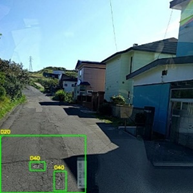
\includegraphics[width=0.23\textwidth]{images/figure9-a-1}}\hfill
                \subfloat[MobileNet+YOLOv4]{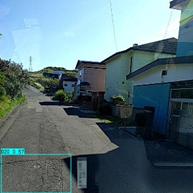
\includegraphics[width=0.23\textwidth]{images/figure9-a-2}}\hfill
                \subfloat[EfficientDet]{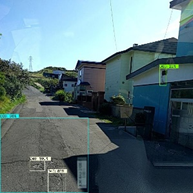
\includegraphics[width=0.23\textwidth]{images/figure9-a-3}}\hfill
                \subfloat[Faster R-CNN]{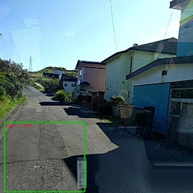
\includegraphics[width=0.23\textwidth]{images/figure9-a-4}}\\
                \subfloat[SSD MobileNet]{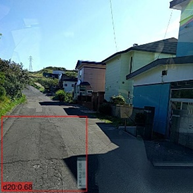
\includegraphics[width=0.23\textwidth]{images/figure9-a-5}}\hfill
                \subfloat[RetinaNet]{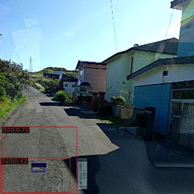
\includegraphics[width=0.23\textwidth]{images/figure9-a-6}}\hfill
                \subfloat[YOLOv5]{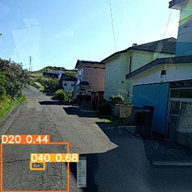
\includegraphics[width=0.23\textwidth]{images/figure9-a-7}}\hfill
                \subfloat[CAYOLO]{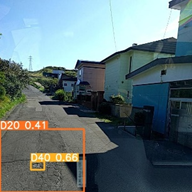
\includegraphics[width=0.23\textwidth]{images/figure9-a-8}}
            \end{minipage}
        }
        \\
        % 第二组 (b)
        \subfloat{
            \parbox[l]{0.05\textwidth}{(b)\label{fig:9-b}}
            \begin{minipage}{0.95\textwidth}
                \subfloat[Ground-truth box]{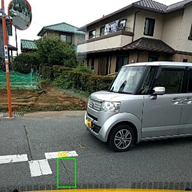
\includegraphics[width=0.23\textwidth]{images/figure9-b-1}}\hfill
                \subfloat[MobileNet+YOLOv4]{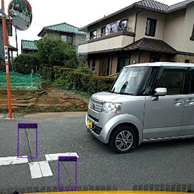
\includegraphics[width=0.23\textwidth]{images/figure9-b-2}}\hfill
                \subfloat[EfficientDet]{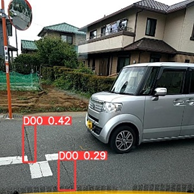
\includegraphics[width=0.23\textwidth]{images/figure9-b-3}}\hfill
                \subfloat[Faster R-CNN]{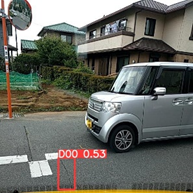
\includegraphics[width=0.23\textwidth]{images/figure9-b-4}}\\
                \subfloat[SSD MobileNet]{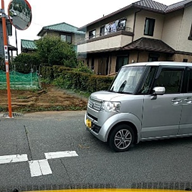
\includegraphics[width=0.23\textwidth]{images/figure9-b-5}}\hfill
                \subfloat[RetinaNet]{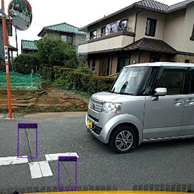
\includegraphics[width=0.23\textwidth]{images/figure9-b-6}}\hfill
                \subfloat[YOLOv5]{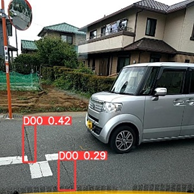
\includegraphics[width=0.23\textwidth]{images/figure9-b-7}}\hfill
                \subfloat[CAYOLO]{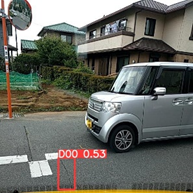
\includegraphics[width=0.23\textwidth]{images/figure9-b-8}}
            \end{minipage}
        }
        \\
        % 第三组 (c)
        \subfloat{
            \parbox[l]{0.05\textwidth}{(c)\label{fig:9-c}}
            \begin{minipage}{0.95\textwidth}
                \subfloat[Ground-truth box]{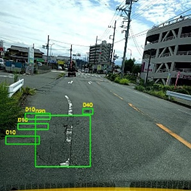
\includegraphics[width=0.23\textwidth]{images/figure9-c-1}}\hfill
                \subfloat[MobileNet+YOLOv4]{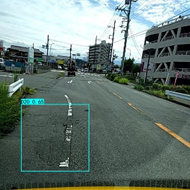
\includegraphics[width=0.23\textwidth]{images/figure9-c-2}}\hfill
                \subfloat[EfficientDet]{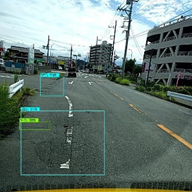
\includegraphics[width=0.23\textwidth]{images/figure9-c-3}}\hfill
                \subfloat[Faster R-CNN]{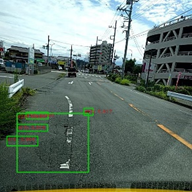
\includegraphics[width=0.23\textwidth]{images/figure9-c-4}}\\
                \subfloat[SSD MobileNet]{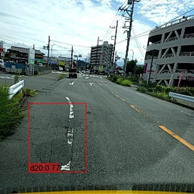
\includegraphics[width=0.23\textwidth]{images/figure9-c-5}}\hfill
                \subfloat[RetinaNet]{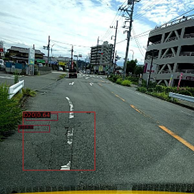
\includegraphics[width=0.23\textwidth]{images/figure9-c-6}}\hfill
                \subfloat[YOLOv5]{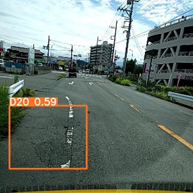
\includegraphics[width=0.23\textwidth]{images/figure9-c-7}}\hfill
                \subfloat[CAYOLO]{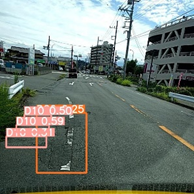
\includegraphics[width=0.23\textwidth]{images/figure9-c-8}}
            \end{minipage}
        }

        \caption{Comparison of different network test results.\label{fig:9}}
    \end{figure}

    The mAP values of each network's training process are shown in \autoref{fig:6}. According to \autoref{fig:6}, the CAYOLO network suggested in this article has considerably improved the detection performance of various networks. The CAYOLO network provided in this paper is more stable and effective than several other networks.

    \begin{table}[H]
        \caption{Individual training model parameters and test single image time.\label{tab:3}}
        \begin{tabularx}{\textwidth}{CCC}
            \toprule
            \textbf{Model}   & \textbf{Paramerters} & \textbf{Avg time per image} \\
            \midrule
            MobileNet+YOLOv4 & 51.1MB               & 19.6ms                      \\
            EfficientDet     & 15.0MB               & 34.7ms                      \\
            Faster R-CNN     & 360MB                & 92.4ms                      \\
            SSD MobileNet    & 23.8MB               & 44.3ms                      \\
            RetinaNet        & 277MB                & 12.95ms                     \\
            YOLOv5           & 14.2MB               & 11.1ms                      \\
            \bottomrule
        \end{tabularx}
    \end{table}


    \autoref{tab:3} shows the model size and time parameters of the test dataset obtained by training with each network, and the test image size is set to 640×640. The table shows that the model obtained by training with YOLOv5 is the smallest, while the model obtained by training with Faster R-CNN with resnet101 as the backbone is the largest, with a single model reaching 360MB. The time used to test a single image in Compared with YOLOv5, the average detection time of CAYOLO for a single image is improved by 8.82\%, sacrificing a petite model size. They are bringing an increase in model testing speed.

    \autoref{tab:4} shows that although the detection speed is slower, the F1-Score in [44] is similar to the CAYOLO result. In [46], the maximum value is obtained when the IoU is 0.75, but this method takes a long time. The highest F1 value of 0.5814 was attained in [41] using the pre-training model and extensive training sets. \autoref{tab:4} demonstrates that when the IoU is 0.75, the mAP value of each network decrease by at least half. As a result, when the IoU is 0.5, this study performs model training and evaluation. This study proposed in this work can achieve good performance and the quickest detection speed among the current methods.


    \begin{table}[H]
        \caption{Comparison of the results of CAYOLO and different papers'.\label{tab:4}}
        \begin{tabularx}{\textwidth}{CCCCC}
            \toprule
            \textbf{Methods}       & \textbf{mAP@.5} & \textbf{mAP@.75} & \textbf{F1-score} & \textbf{Avg test time per image} \\
            \midrule
            Binyi Su[52]           & 0.517           & -                & -                 & 60.9ms                           \\
            \mbox{Minh-Tu Cao[45]} & 0.547           & 0.249            & 0.5145            & 17s `                             \\
            Naddaf-Sh[43]          & 0.542           & 0.152            & 0.566             & 17.8ms                           \\
            Mandal[40]             & -               & -                & 0.5814/0.5751     & 15.3ms                           \\
            YOLOv5                 & 0.519           & 0.227            & 0.545             & 11.1ms                           \\
            CAYOLO                 & 0.558           & 0.241            & 0.567             & 10.2ms                           \\
            \bottomrule
        \end{tabularx}
    \end{table}

    \subsection{Road Damage Detection Results in Different Countries}

    This section conducts experiments using the models trained by YOLOv5 and CAYOLO, respectively, in the previous sections to assess whether the proposed model approach can adapt to the road conditions in various nations. The datasets used are the training images of the Czech Republic and India provided by RDD-2020 and the 1981 images collected by this research team from the Hunan Province of China. These data are randomly divided in the ratio of 8:1:1 to assess the model's effectiveness for detecting roads in various nations after the five more irrelevant categories have been discarded, similarly.

    \autoref{fig:10} and \autoref{fig:11} display the fluctuation in mAP values for each country during the training process and the PR plots for the detection of the test set, respectively. Figure~\autoref{fig:10-a} shows that using CAYOLO is more stable and better in the training process; Figure~\autoref{fig:10-b} illustrates that using YOLOv5 to train the Czech road can stabilize earlier compared to CAYOLO, but using CAYOLO can get better results; Figure~\autoref{fig:10-c} proves that using YOLOv5 can stabilize earlier, and after training up to 400 epochs, the two can be used interchangeably. The two networks can produce virtually the same outputs after 400 training epochs. Figure~\hyperref[fig:11-a]{11(a)} exemplifies that when testing the Indian road images, CAYOLO can achieve better performance than YOLOv5 in detecting D10 class damages because the total number of D10 class damages is too minimal, the road conditions are more complicated, and the network has difficulty learning the relevant features of D10 class damages; Figure~\hyperref[fig:11-b]{11(b)} shows that when testing the Czech road images, CAYOLO can achieve better performance in detecting D10 and D40 damages; and YOLOv5 can achieve better performance in detecting D00 and D20 categories of damages; Figure~\hyperref[fig:11-c]{11(c)} demonstrates that when examining Chinese road photos, the two network models can almost always perform equally well. In general, CAYOLO, used in this study, can produce better road detection outcomes.

    \begin{figure}[H]
        \captionsetup[subfloat]{labelformat=empty}

        \subfloat{
            \parbox[c]{0.2\textwidth}{(a)\label{fig:10-a}}
            \begin{minipage}{0.6\textwidth}
                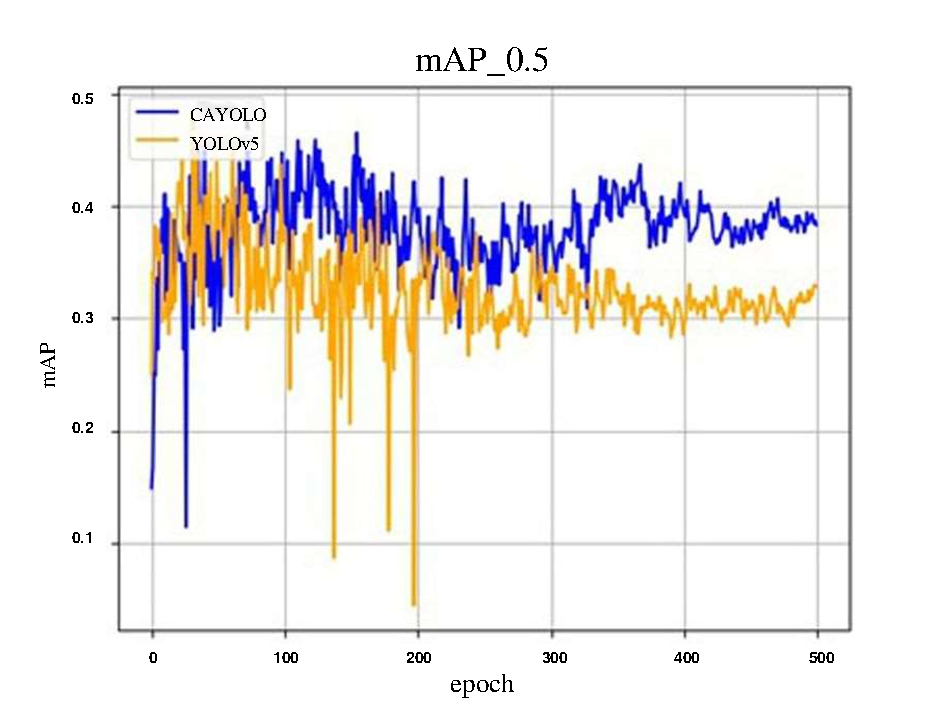
\includegraphics[width=10cm]{images/figure10-a}
            \end{minipage}}
        \\
        \subfloat{
            \parbox[c]{0.2\textwidth}{(b)\label{fig:10-b}}
            \begin{minipage}{0.6\textwidth}
                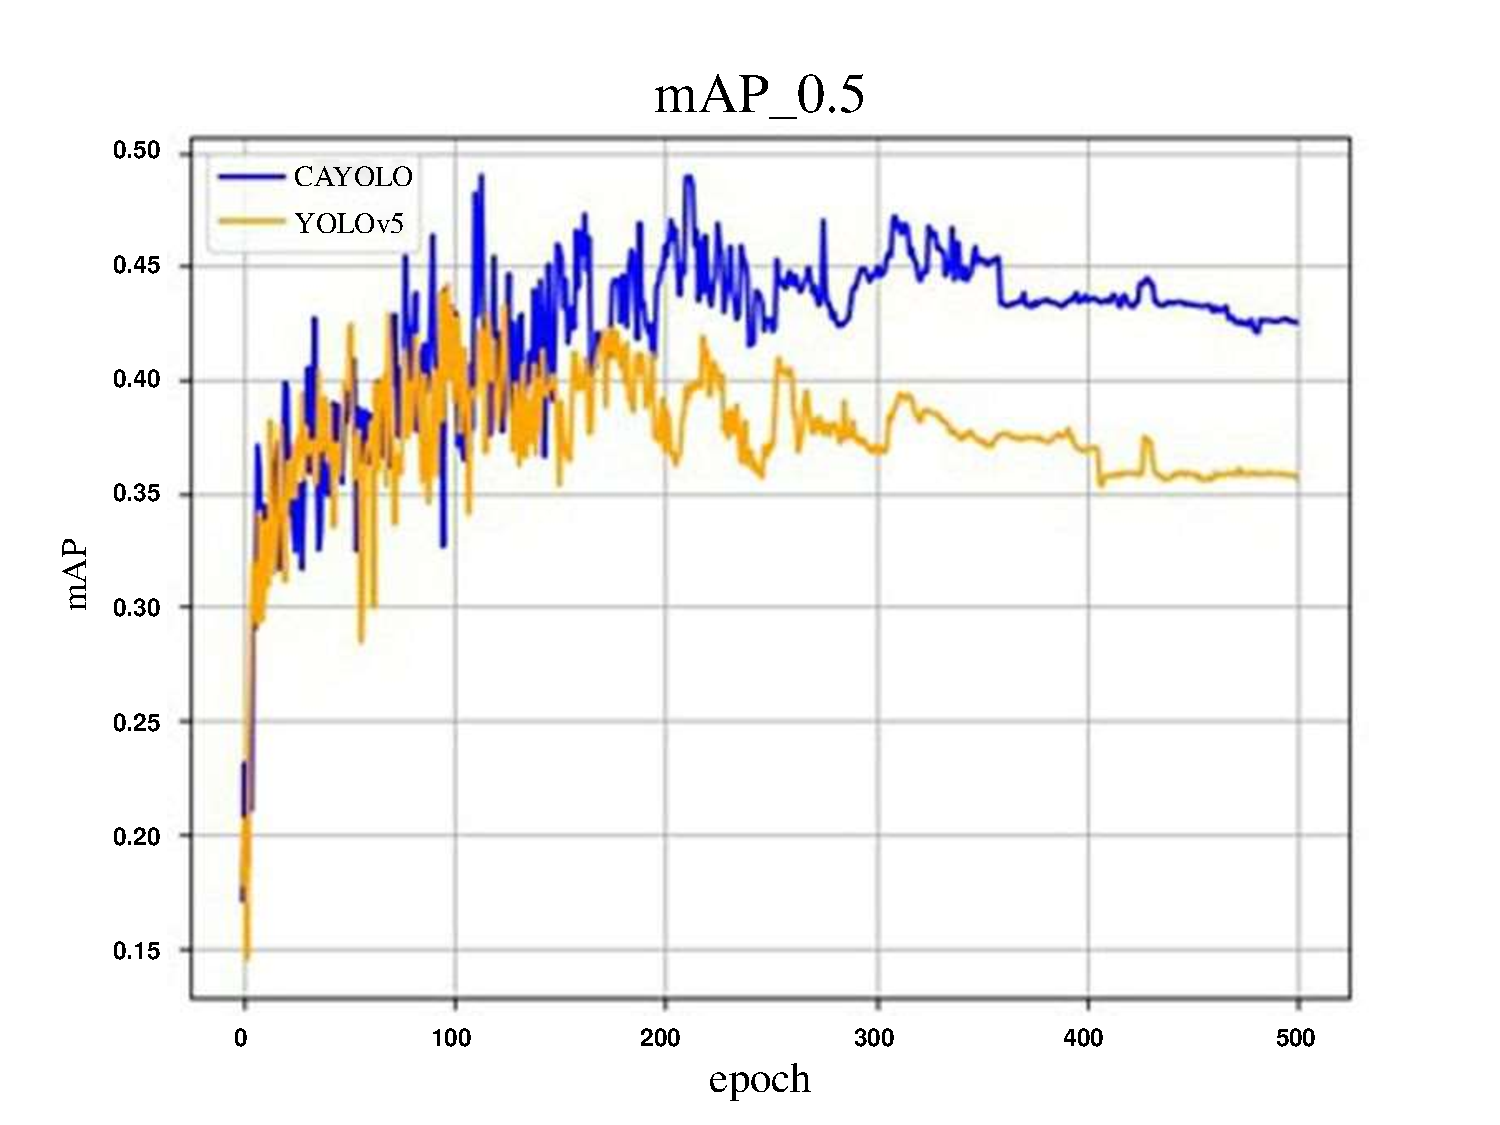
\includegraphics[width=10cm]{images/figure10-b}
            \end{minipage}}
        \\
        \subfloat{
            \parbox[c]{0.2\textwidth}{(c)\label{fig:10-c}}
            \begin{minipage}{0.6\textwidth}
                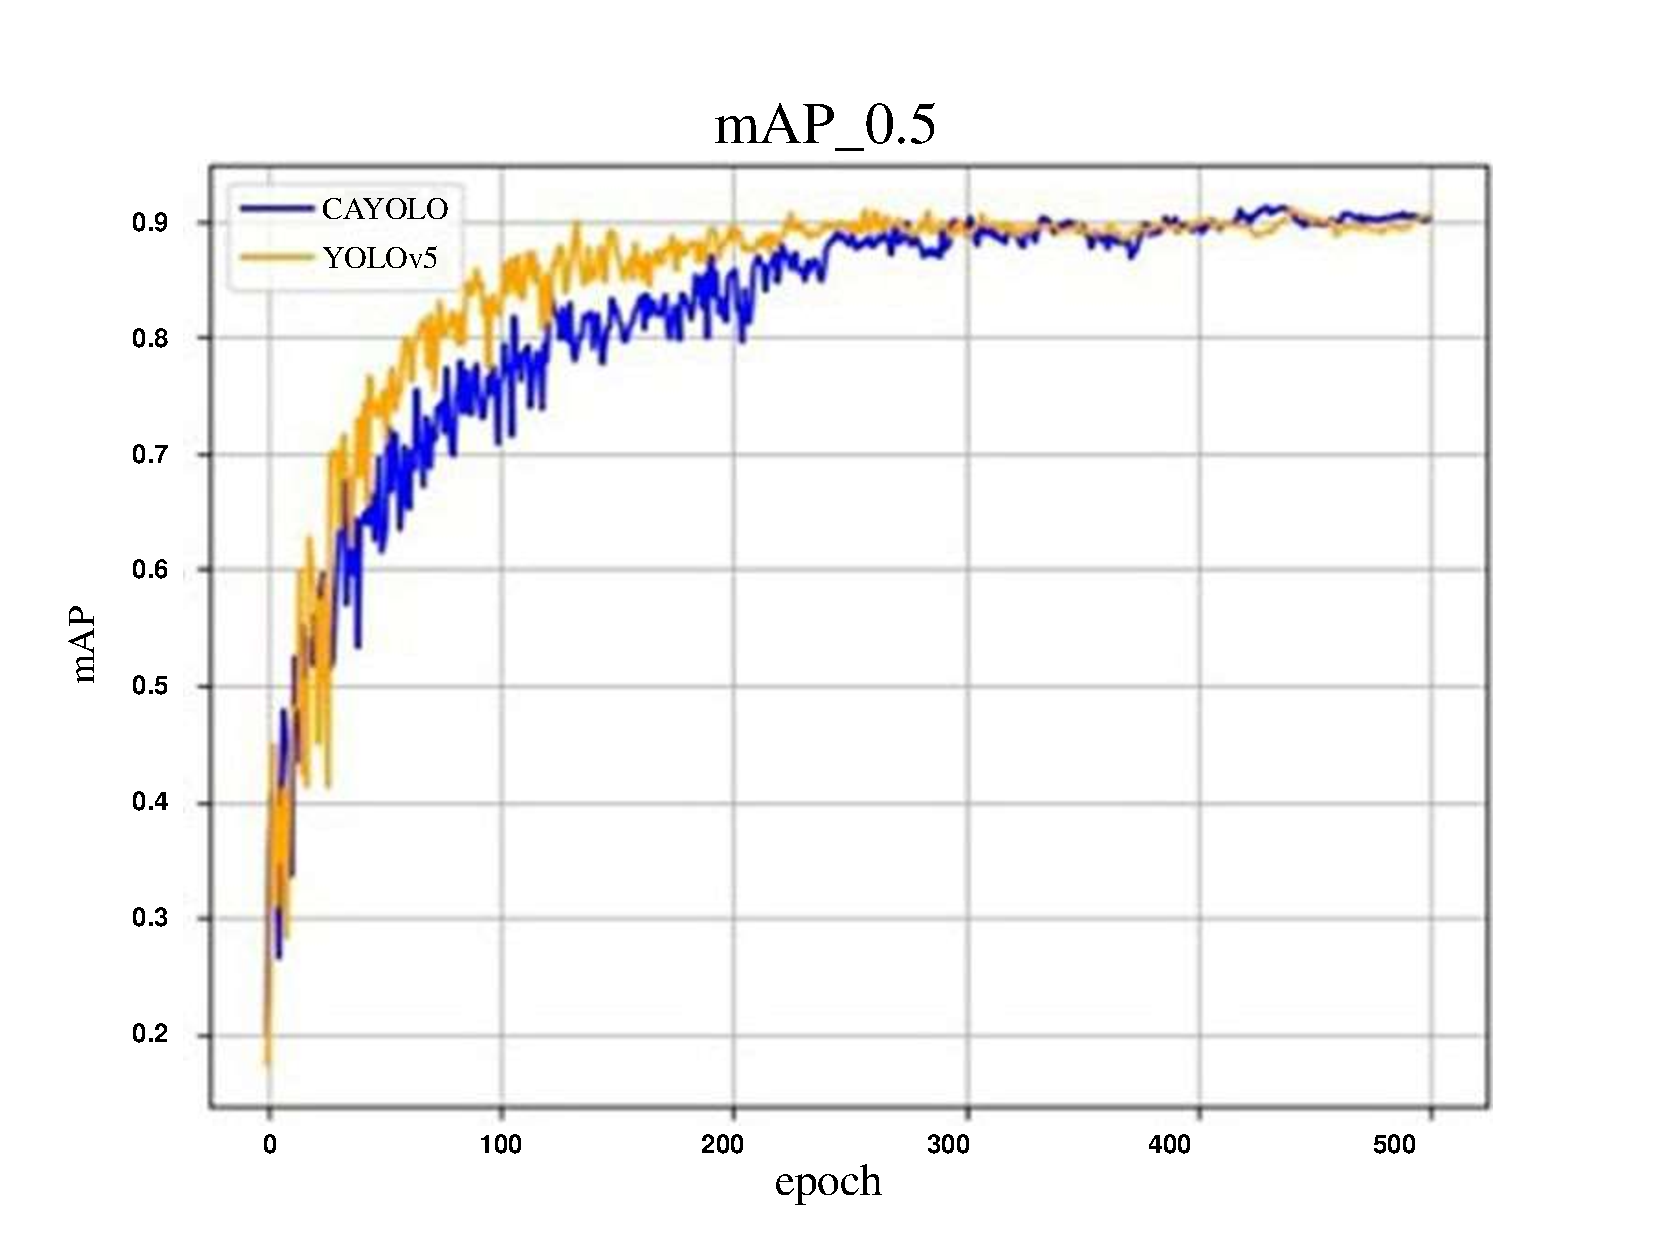
\includegraphics[width=10cm]{images/figure10-c}
            \end{minipage}}

        \captionsetup[subfloat]{labelformat=parens}
        \caption{(a) (b) (c) is the mAP changes during training for the Indian, Czech, and Chinese road images.\label{fig:10}}
    \end{figure}

    \begin{figure}[H]
        \centering
        \captionsetup[subfloat]{labelformat=empty,justification=centering}

        \subfloat{
            \parbox[c]{0.05\textwidth}{(a)\label{fig:11-a}}
            \begin{minipage}{0.95\textwidth}
                \subfloat{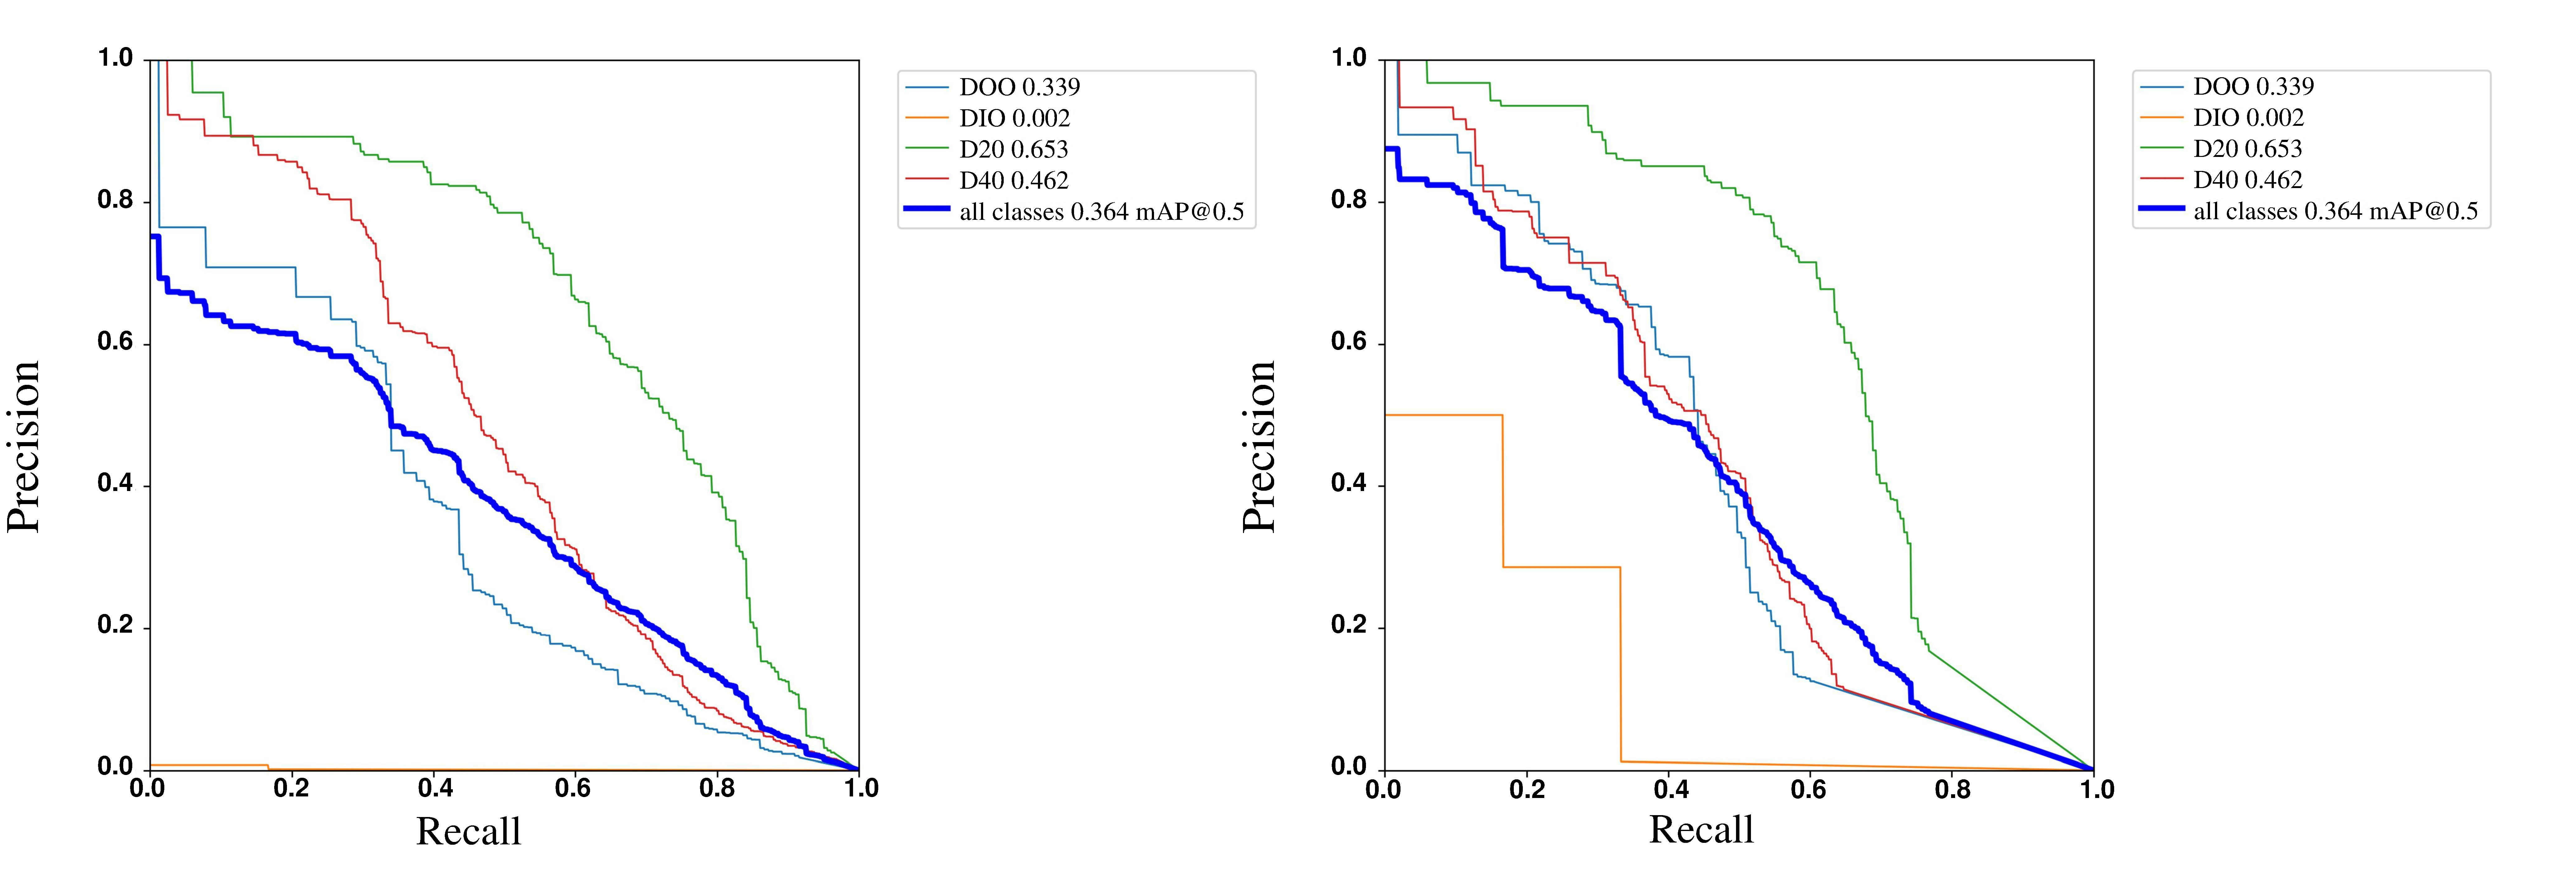
\includegraphics[width=0.95\textwidth]{images/figure11-a}}
            \end{minipage}
        }
        \\
        \subfloat{
            \parbox[c]{0.05\textwidth}{(b)\label{fig:11-b}}
            \begin{minipage}{0.95\textwidth}
                \subfloat{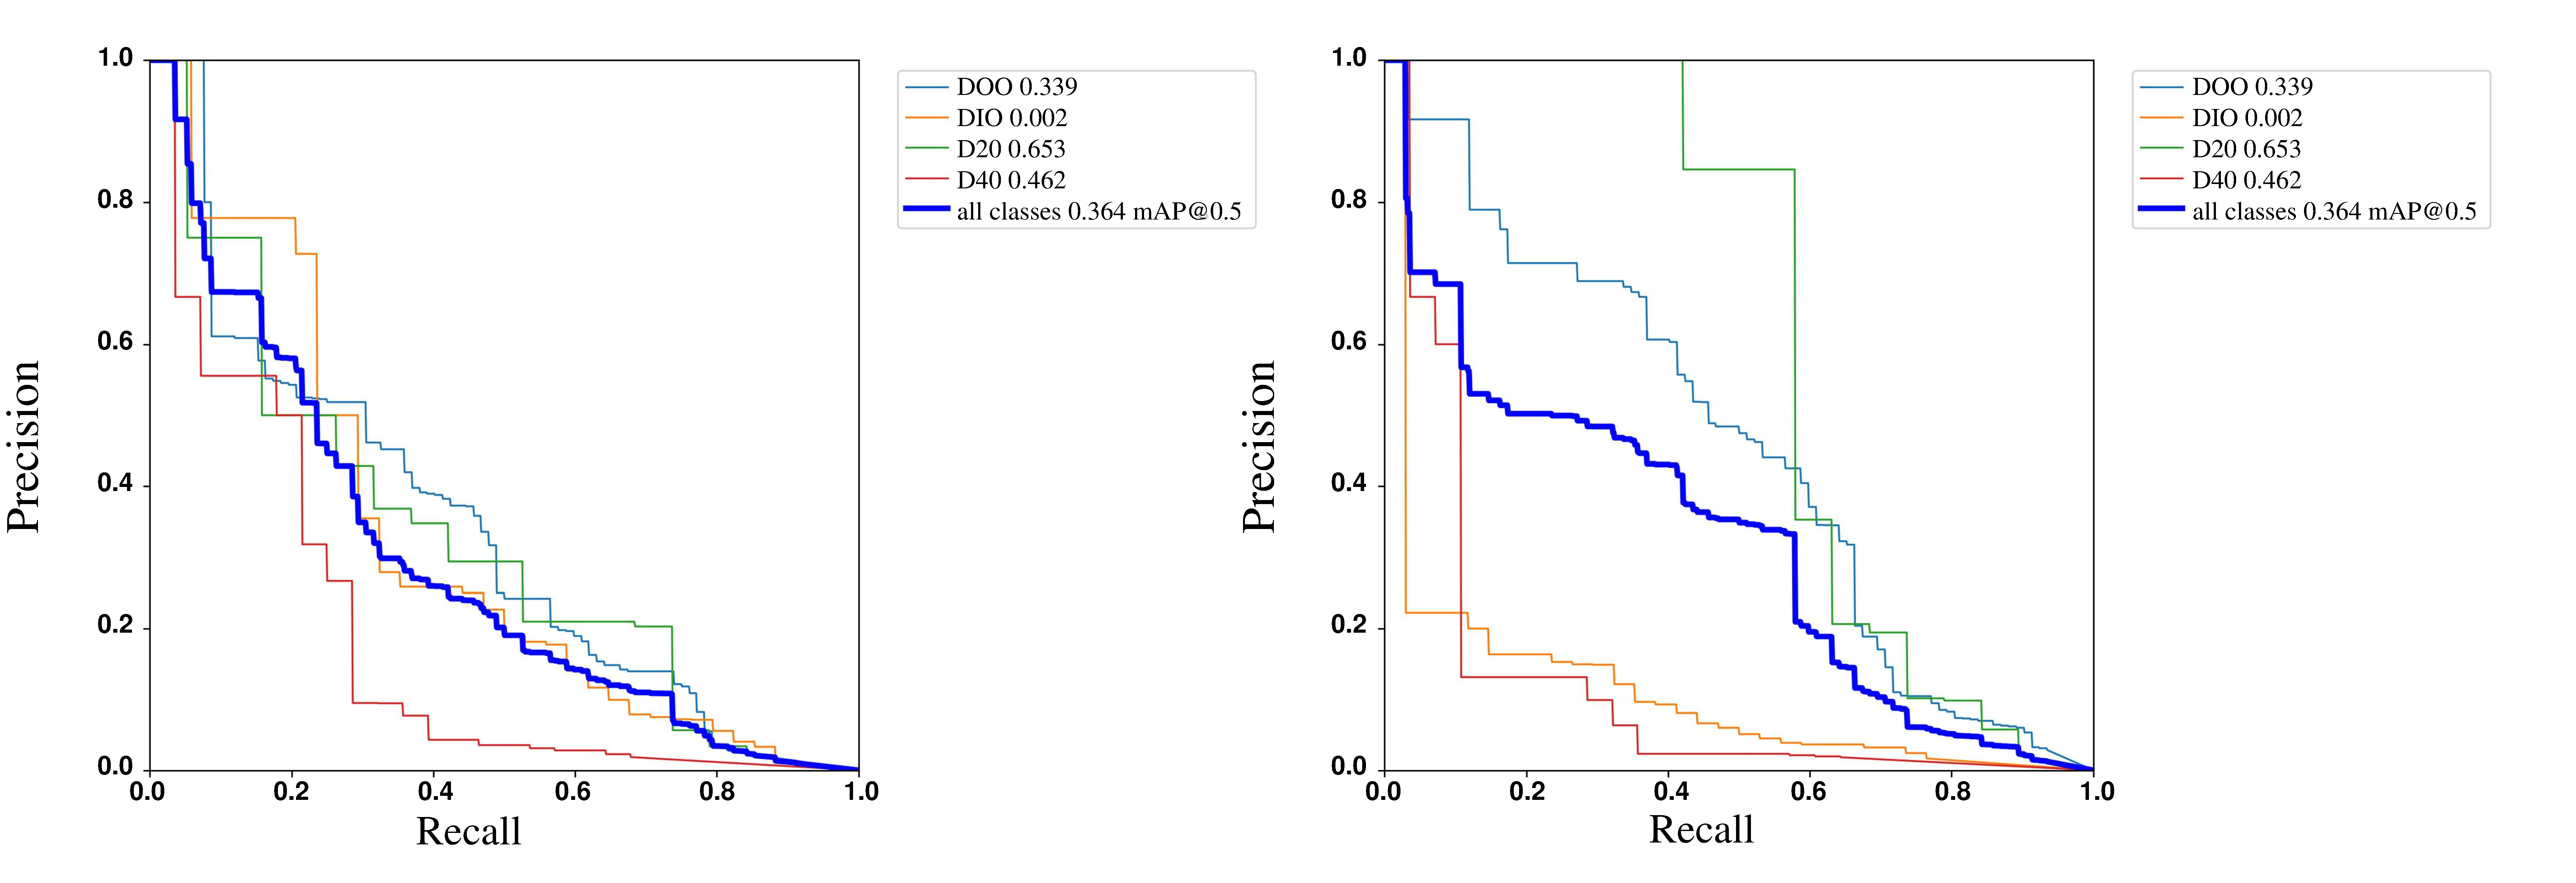
\includegraphics[width=0.95\textwidth]{images/figure11-b}}
            \end{minipage}
        }
        \\
        \subfloat{
            \parbox[c]{0.05\textwidth}{(c)\label{fig:11-c}}
            \begin{minipage}{0.95\textwidth}
                \subfloat{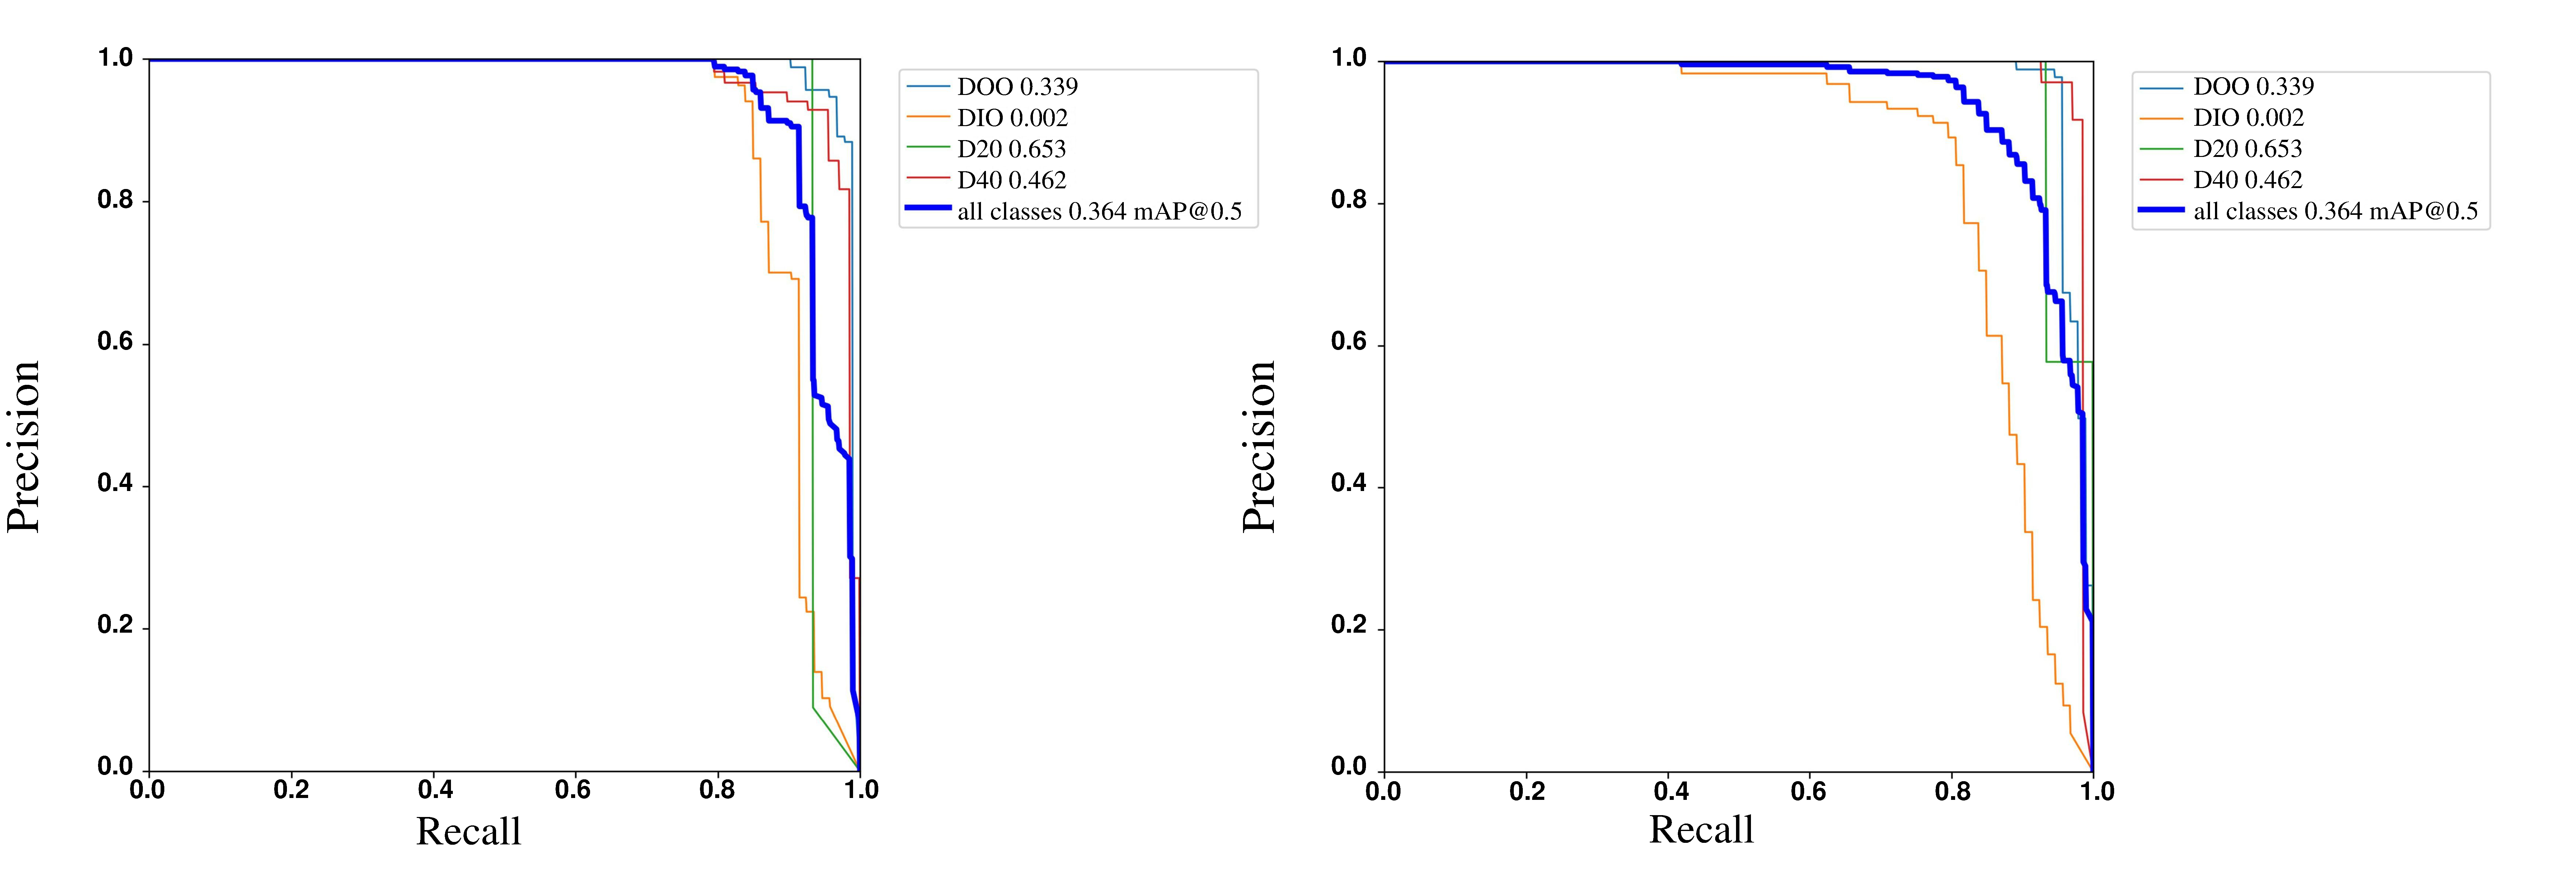
\includegraphics[width=0.95\textwidth]{images/figure11-c}}
            \end{minipage}
        }

        \caption{(a) (b) (c) are PR maps for India, the Czech Republic, and China, respectively, using YOLOv5 on the left and CAYOLO on the right.\label{fig:11}}
    \end{figure}


    In Figure~\hyperref[fig:12-c]{12(c)}, YOLOv5 fails to identify the damage, CAYOLO misidentifies D10 as D40 damage, there are too few D10 damages in the Indian road data, the network has low sensitivity to D10-like damages, and in Figure~\hyperref[fig:12-e]{12(e)}, it is a non-concrete pavement and misidentifies multiple D40 damages. In Figure~\autoref{fig:13-a}, CAYOLO correctly identifies all the damages, while YOLOv5 has some problems in detecting D20 damages; in Figure~\autoref{fig:13-b} and Figure~\autoref{fig:13-e}, YOLOv5 can accurately identify D10 damages while CAYOLO fails to do so. In \autoref{fig:14}, both YOLOv5 and CAYOLO have some deficiencies in detecting D10 damage but present the same performance in detecting other damages.

    We can see that CAYOLO can achieve better detection performance in most cases. CAYOLO utilizes an attention mechanism that can capture directional and channel information, and extract information that is often overlooked as the network deepens. It also uses a double convolution structure with small convolution kernels to extract features of small cracks. In addition, the Ghost Module is used to make the network lightweight and reduce the unnecessary computation brought by traditional convolutions during training. However, there is still significant room for improvement in detecting transverse cracks with CAYOLO. As shown in \autoref{fig:6}, it has oscillation problems in the early stages of training, and in \autoref{tab:4}, its F1-score is slightly lower than some other studies. This is because the CAYOLO model has not achieved a good balance between precision and recall, and there are still some defects in the network's ability to recognize certain diseases. Nevertheless, it has also made good progress in detection speed and some aspects, although there is still some distance to go in improving the F1-score.

    \begin{figure}[H]
        \captionsetup[subfloat]{labelformat=empty}

        \subfloat{\parbox[c]{0.1\textwidth}{(a)\label{fig:12-a}}
            \begin{minipage}{0.9\textwidth}
                \hfill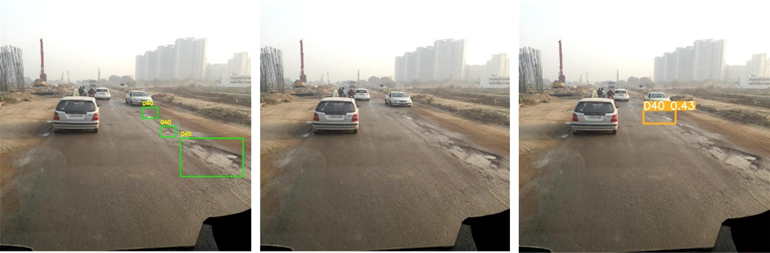
\includegraphics[width=0.9\textwidth]{images/figure12-a}
            \end{minipage}}\\
        \subfloat{\parbox[c]{0.1\textwidth}{(b)\label{fig:12-b}}
            \begin{minipage}{0.9\textwidth}
                \hfill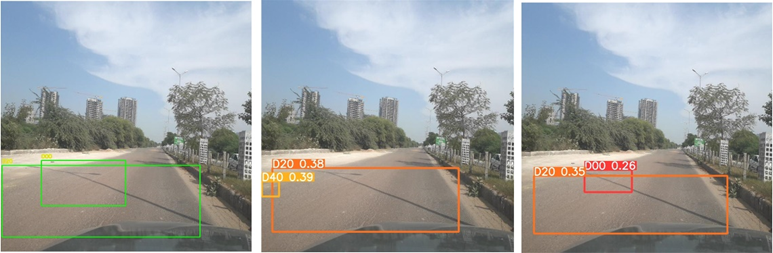
\includegraphics[width=0.9\textwidth]{images/figure12-b}
            \end{minipage}}\\
        \subfloat{\parbox[c]{0.1\textwidth}{(c)\label{fig:12-c}}
            \begin{minipage}{0.9\textwidth}
                \hfill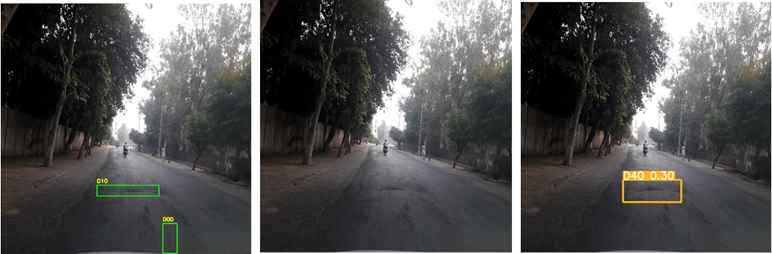
\includegraphics[width=0.9\textwidth]{images/figure12-c}
            \end{minipage}}\\
        \subfloat{\parbox[c]{0.1\textwidth}{(d)\label{fig:12-d}}
            \begin{minipage}{0.9\textwidth}
                \hfill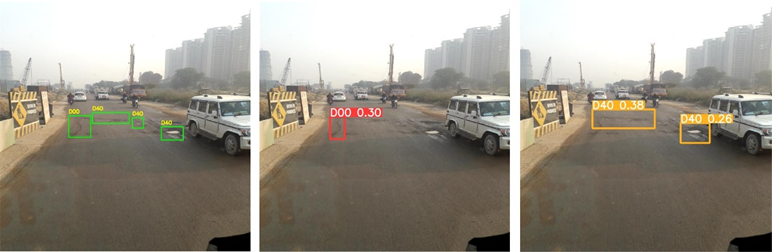
\includegraphics[width=0.9\textwidth]{images/figure12-d}
            \end{minipage}}\\
        \subfloat{\parbox[c]{0.1\textwidth}{(e)\label{fig:12-e}}
            \begin{minipage}{0.9\textwidth}
                \hfill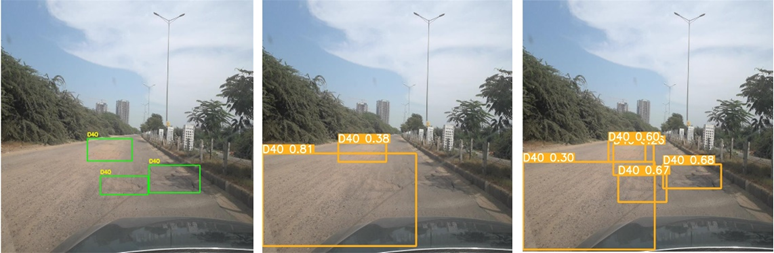
\includegraphics[width=0.9\textwidth]{images/figure12-e}
            \end{minipage}}

        \captionsetup[subfloat]{labelformat=parens}
        \caption{Test Indian Road picture results. The left side is the actual label of the disease; the middle uses the YOLOv5 model test picturel; the right uses the CAYOLO model test picture.\label{fig:12}}
    \end{figure}

    \begin{figure}[H]
        \captionsetup[subfloat]{labelformat=empty}

        \subfloat{\parbox[c]{0.1\textwidth}{(a)\label{fig:13-a}}
            \begin{minipage}{0.9\textwidth}
                \hfill\includegraphics[width=0.9\textwidth]{images/figure13-a}
            \end{minipage}}\\
        \subfloat{\parbox[c]{0.1\textwidth}{(b)\label{fig:13-b}}
            \begin{minipage}{0.9\textwidth}
                \hfill\includegraphics[width=0.9\textwidth]{images/figure13-b}
            \end{minipage}}\\
        \subfloat{\parbox[c]{0.1\textwidth}{(c)\label{fig:13-c}}
            \begin{minipage}{0.9\textwidth}
                \hfill\includegraphics[width=0.9\textwidth]{images/figure13-c}
            \end{minipage}}\\
        \subfloat{\parbox[c]{0.1\textwidth}{(d)\label{fig:13-d}}
            \begin{minipage}{0.9\textwidth}
                \hfill\includegraphics[width=0.9\textwidth]{images/figure13-d}
            \end{minipage}}\\
        \subfloat{\parbox[c]{0.1\textwidth}{(e)\label{fig:13-e}}
            \begin{minipage}{0.9\textwidth}
                \hfill\hfill\includegraphics[width=0.9\textwidth]{images/figure13-e}
            \end{minipage}}

        \captionsetup[subfloat]{labelformat=parens}
        \caption{Test Indian Road picture results. The left side is the actual label of the disease; the middle uses the YOLOv5 model test picturel; the right uses the CAYOLO model test picture.\label{fig:13}}
    \end{figure}

    \begin{figure}[H]
        \captionsetup[subfloat]{labelformat=empty}

        \subfloat{\parbox[c]{0.1\textwidth}{(a)\label{fig:14-a}}
            \begin{minipage}{0.9\textwidth}
                \hfill\includegraphics[width=0.9\textwidth]{images/figure14-a}
            \end{minipage}}\\
        \subfloat{\parbox[c]{0.1\textwidth}{(b)\label{fig:14-b}}
            \begin{minipage}{0.9\textwidth}
                \hfill\includegraphics[width=0.9\textwidth]{images/figure14-b}
            \end{minipage}}\\
        \subfloat{\parbox[c]{0.1\textwidth}{(c)\label{fig:14-c}}
            \begin{minipage}{0.9\textwidth}
                \hfill\includegraphics[width=0.9\textwidth]{images/figure14-c}
            \end{minipage}}\\
        \subfloat{\parbox[c]{0.1\textwidth}{(d)\label{fig:14-d}}
            \begin{minipage}{0.9\textwidth}
                \hfill\includegraphics[width=0.9\textwidth]{images/figure14-d}
            \end{minipage}}\\
        \subfloat{\parbox[c]{0.1\textwidth}{(e)\label{fig:14-e}}
            \begin{minipage}{0.9\textwidth}
                \hfill\includegraphics[width=0.9\textwidth]{images/figure14-e}
            \end{minipage}}

        \captionsetup[subfloat]{labelformat=parens}
        \caption{Test Indian Road picture results. The left side is the actual label of the disease; the middle uses the YOLOv5 model test picturel; the right uses the CAYOLO model test picture.\label{fig:14}}
    \end{figure}


    \section{Discussion and Conclusions}


    The DBC3 and CAC3 modules are created to construct the CAYOLO deep neural network according to the damage's characteristics. The network in this article focuses on the extraction of pavement crack features. The designed network model is compared with several mainstream algorithms in the field of road damage detection. The results show that using the CAYOLO network model can achieve significantly improved results on the publicly available dataset RDD-2020, with an mAP value of 68.86\% for the alligator crack damage. CAYOLO also achieves the fastest detection speed among the same type of networks, with the time taken to detect a single image being 10.2ms. The trained YOLOv5 and CAYOLO models are retrained separately using data from several nations. The performance on Chinese road photographs is the best, with mAP reaching 94.9\%, thus demonstrating the CAYOLO's ability to deliver noticeably enhanced results. Additionally, we'll make the relevant information we've gathered available to the public for use by other academics and keep gathering and updating the dataset.

    We may infer from the trials that most network models challenge to extract lateral fractures. Thus in the subsequent studies, we must concentrate on enhancing the algorithm's power to do so. To increase the effectiveness of road damage identification in multiple nations, we will keep looking for better road damage detection methods in the future. Additionally, the dataset's size and quality must be increased, and the photos that were incorrectly labeled must be fixed. By doing so, the effect of mislabeling on the network can be partly mitigated. More data could be collected in the future via smartphones or cameras installed on buses. The government might also encourage citizens to capture road photographs for research by adopting suitable welfare policies.


%%%%%%%%%%%%%%%%%%%%%%%%%%%%%%%%%%%%%%%%%%
    \vspace{6pt}


%%%%%%%%%%%%%%%%%%%%%%%%%%%%%%%%%%%%%%%%%%
    \authorcontributions{
        Conceptualization, Shuo.Z., S.C. and Z.L.; methodology, Z.L.; validation, Shuo.Z., S.C. and Z.L; formal analysis, Sha.Z.; investigation, Y.Z.T.; resources, Z.L.; data curation, Shuo.Z. and Z.L.; writing—original draft preparation, Z.L.; writing—review and editing, Shuo.Z. and Z.L.; visualization, Shuo.Z.; supervision, S.B.C.; project administration, S.B.C. All authors have read and agreed to the published version of the manuscript.
    }

%    \funding{Please add: ``This research received no external funding'' or ``This research was funded by NAME OF FUNDER grant number XXX.'' and and ``The APC was funded by XXX''. Check carefully that the details given are accurate and use the standard spelling of funding agency names at \url{https://search.crossref.org/funding}, any errors may affect your future funding.}

    \institutionalreview{Not applicable.}

    \informedconsent{Not applicable.}

    \dataavailability{The data presented in this study are available upon request from the corresponding author.}

    \conflictsofinterest{The authors declare no conflicts of interest.}


%%%%%%%%%%%%%%%%%%%%%%%%%%%%%%%%%%%%%%%%%%
%\isPreprints{} % If the paper is ``preprints'', please uncomment this parenthesis.
%\printendnotes[custom] % Un-comment to print a list of endnotes

        \reftitle{References}

% Please provide either the correct journal abbreviation (e.g. according to the “List of Title Word Abbreviations” http://www.issn.org/services/online-services/access-to-the-ltwa/) or the full name of the journal.
% Citations and References in Supplementary files are permitted provided that they also appear in the reference list here.

%=====================================
% References, variant A: external bibliography
%=====================================
        \bibliography{references}

%=====================================
% References, variant B: internal bibliography
%=====================================

% ACS format
%        \isAPAandChicago{}{%
%            \begin{thebibliography}{999}
%
%                \bibitem[Author1(year)]{ref-journal}
%                Author~1, T. The title of the cited article. {\em Journal Abbreviation} {\bf 2008}, {\em 10}, 142--149.
%
%                \bibitem[Author2(year)]{ref-book1}
%                Author~2, L. The title of the cited contribution. In {\em The Book Title}; Editor 1, F., Editor 2, A., Eds.; Publishing House: City, Country, 2007; pp. 32--58.
%
%                \bibitem[Author1 and Author2 (year)]{ref-book2}
%                Author 1, A.; Author 2, B. \textit{Book Title}, 3rd ed.; Publisher: Publisher Location, Country, 2008; pp. 154--196.
%
%                \bibitem[Author4(year)]{ref-unpublish}
%                Author 1, A.B.; Author 2, C. Title of Unpublished Work. \textit{Abbreviated Journal Name} year, \textit{phrase indicating stage of publication (submitted; accepted; in press)}.
%
%                \bibitem[Author8(year)]{ref-url}
%                Title of Site. Available online: URL (accessed on Day Month Year).
%
%                \bibitem[Author6(year)]{ref-proceeding}
%                Author 1, A.B.; Author 2, C.D.; Author 3, E.F. Title of presentation. In Proceedings of the Name of the Conference, Location of Conference, Country, Date of Conference (Day Month Year); Abstract Number (optional), Pagination (optional).
%
%                \bibitem[Author7(year)]{ref-thesis}
%                Author 1, A.B. Title of Thesis. Level of Thesis, Degree-Granting University, Location of University, Date of Completion.
%            \end{thebibliography}
%        }


% If authors have biography, please use the format below
%\section*{Short Biography of Authors}
%\bio
%{\raisebox{-0.35cm}{\includegraphics[width=3.5cm,height=5.3cm,clip,keepaspectratio]{Definitions/author1.pdf}}}
%{\textbf{Firstname Lastname} Biography of first author}
%
%\bio
%{\raisebox{-0.35cm}{\includegraphics[width=3.5cm,height=5.3cm,clip,keepaspectratio]{Definitions/author2.jpg}}}
%{\textbf{Firstname Lastname} Biography of second author}

% For the MDPI journals use author-date citation, please follow the formatting guidelines on http://www.mdpi.com/authors/references
% To cite two works by the same author: \citeauthor{ref-journal-1a} (\citeyear{ref-journal-1a}, \citeyear{ref-journal-1b}). This produces: Whittaker (1967, 1975)
% To cite two works by the same author with specific pages: \citeauthor{ref-journal-3a} (\citeyear{ref-journal-3a}, p. 328; \citeyear{ref-journal-3b}, p.475). This produces: Wong (1999, p. 328; 2000, p. 475)

%%%%%%%%%%%%%%%%%%%%%%%%%%%%%%%%%%%%%%%%%%
%% for journal Sci
%\reviewreports{\\
%Reviewer 1 comments and authors’ response\\
%Reviewer 2 comments and authors’ response\\
%Reviewer 3 comments and authors’ response
%}
%%%%%%%%%%%%%%%%%%%%%%%%%%%%%%%%%%%%%%%%%%
        \PublishersNote{}
%\isPreprints{} % If the paper is ``preprints'', please uncomment this parenthesis.
\end{document}

